\documentclass[conference]{IEEEtran}

\usepackage{listings}
\usepackage{epsfig}
\usepackage{url}
\usepackage{cite}
\usepackage{fancybox}
\usepackage{amsmath}
\usepackage{amssymb}
\usepackage{amsfonts}
\usepackage{amsthm}
\usepackage{tikz}
\usepackage{multirow}
\usepackage{balance}
\usepackage{enumitem}
\usepackage{graphicx}
\usepackage{pdfpages}
\usepackage{subfig}
\usepackage[ruled,linesnumbered]{algorithm2e}

\usepackage[scaled]{beramono}
\usepackage[T1]{fontenc}

\usepackage[english]{babel} % handle hyphenation

\usepackage{amssymb}

\let\oldemptyset\emptyset
\let\emptyset\varnothing

\lstset{
numbers=left,
frame=single,
language=C,
basicstyle=\fontfamily{fvm}\scriptsize,
showlines=true
%xleftmargin=.2\textwidth, xrightmargin=.2\textwidth,
}

\newcommand{\highlight}[1]{\colorbox{yellow}{\textbf{#1}}}
\newcommand{\fixme}[1]{\highlight{FIXME:} \emph{#1}}
\newcommand{\todo}[1]{\highlight{TODO:} \emph{#1}}
\newcommand{\Qinkun}[1]{\highlight{Qinkun's Response:} \emph{#1}}

\newcommand{\tool}{TANA}
\renewcommand{\tool}{CleverHans}
\renewcommand{\tool}{Cygne}
\renewcommand{\tool}{Do-Re-Mi}
\renewcommand{\tool}{Ta-fa Te-fe}
\renewcommand{\tool}{Ti-ri-ti-ri}
\renewcommand{\tool}{Du-Ta-De-Ta}
\renewcommand{\tool}{Abacus}
\newcommand{\tana}{\tool}

\begin{document}

%\title{\tool{}: Precise Fine-grained Side-channel Information Leakage Quantification in Binaries}
\title{\tool{}: Precise, Scalable, and Fine-grained Side-channel Information Leakage Quantification for Production Software}
\author{Anonymous}

\maketitle

\begin{abstract}
Side-channel attacks allow adversaries to infer sensitive information
based on non-functional characteristics.  Existing work on
software  side-channel detections can identify many potential
vulnerabilities.  %side-channel leakage sites.
However, in practice many such vulnerabilities leak negligible amount of sensitive information
and thus developers are often reluctant to address them. 
%Those leakage sites can leak one bit, two bits, or many bits.
On the other hand,
no existing tools can precisely report the number of leaked
bits for each leakage site, for production systems.

To overcome this limitation, we propose a novel method to precisely
quantify the leaked information from side-channel vulnerabilities.  We
model each leakage as a constraint and use these constraints to
divide the input space into subsets such that  %.  Among those subsets,
only one subset satisfies every constraint.  %As we discuss later,
The cardinality of the subset corresponds to the amount of leaked
information from those leakages.
We use symbolic execution to
generate the constraints, 
%% It is widely believed that symbolic
%% execution is expensive in terms of performance. We systematically
%% analyze the bottlenecks of the current dynamic symbolic execution
%% approach and make it scalable to real-world cryptosystems.
and then run Monte Carlo sampling to estimate the number of
leaked information.  % for each detected vulnerability.
By using   %With the help of
the Central Limit Theorem, we can also give the error bound for
estimation.

We have implemented the above technique in a tool called \tool{},
which can not only find the side-channel vulnerabilities but also
estimate how many bits are leaked.  \tool{} outperforms existing
dynamic side-channel detection tools in terms of performance and
accuracy. Also, \tool{} can report a very fined-grained vulnerability
leakage information. 
%% Compared to existing abstract interpretation
%% approaches that can only give upper leakage bounds, the information
%% reported by our tool is more useful for developers to identify the
%% severity level of each side-channel vulnerability.
 We evaluated 
\tool{} on OpenSSL, MbedTLS, and found several severe side-channel
vulnerabilities.
\fixme{Need to update the rest of the abstract after the evaluation section is done.}
Compared with previous research, the results are
surprisingly different.  First, it shows that most of the reported
vulnerabilities are hard to exploit in practice.  Second, we also find
several sensitive vulnerabilities that are missed by existing tools.
We confirmed those vulnerabilities with manual checks and software
developers.
    %% which are confirmed with manual checks and software developpers. 

\end{abstract}


\IEEEpeerreviewmaketitle
\pagenumbering{arabic}
\pagestyle{plain}

\section{Introduction}
%% side channels are important
Side channels are inevitable in modern computer systems as the sensitive information 
may be leaked by many kinds of inadvertent behaviors, 
such as power, electromagnetic radiation and even 
sound~\cite{agrawal2002side,kar20178,chari1999towards,217605,genkin2014rsa}. 
Among them, software-based side channels, such as cache attacks, memory page attacks,
and controlled-channel attacks, are especially common 
and have been studied for years~\cite{7163052, 217543, 217589, lee2017inferring, 191010}. 
These vulnerabilities result from vulnerable software and shared hardware components.
By observing the outputs or hardware behaviors, attackers can
infer the program execution flow that manipulate secrets and 
guess the secrets such as encryption keys~\cite{Osvik2006}.

%% to deal with side channels, we can protect or detect them and detection is better
Various countermeasures have been proposed to defend against 
software-based side-channel attacks. Hardware level solutions, 
including reducing shared resources, adopting oblivious RAM, and using
transnational memory~\cite{203878,217537} need new hardware features or changes
to modern complex computer systems, which is impractical and hard to adopt in 
reality. Therefore, a more promising and universal direction is software countermeasures, 
detecting and eliminating side channel vulnerabilities from code.

Regarding the root cause of software-based side channels, 
many of them are caused by the following two specific types: 
data flow from secrets to load addresses and data flow from secrets to branch conditions.
We call them secret-dependent control-flow and memory-access correspondingly.
Therefore, a central problem is identifying those two code patterns automatically.
Recent works~\cite{203878,217537,Wichelmann:2018:MFF:3274694.3274741,Brotzman19Casym,236338,182946} 
adopt static and dynamic analysis
to detect side-channels.
They can find many potential leak sites in real-world software, 
but fail to report how severe a potential leakage could be. 
Many of the reported vulnerabilities are typically hard to exploit
and leak very little information. For example, DATA~\cite{217537} reports
2,246 potential leakage site for the RSA implementation in OpenSSL\@.
After some inspections, 1,510 are dismissed, but it still
leaves 278 control-flow and 460 data-access patterns. For software
developers, it is hard for them to fix all those vulnerabilities,
let alone the majority of them are negligible.
While some vulnerabilities can be used to recover the full secret
keys~\cite{184415}, many other vulnerabilities prove to be less serious in reality.

To assess the sensitive level of side-channel vulnerabilities, we need a proper 
quantification metric.
Static methods~\cite{182946,5207642}, usually with abstract interpretations, can give a leakage upper bound, 
which is useful to justify the implementation is secure when they report zero or little leakage. 
However, they cannot indicate how serious the leakage is because of over-approximation. 
For example, CacheAudit~\cite{182946} reports that the upper bound leakage of AES-128 exceeds 
the original key size! The dynamic methods take another approach with a concrete input and 
run the program in real environment. Although they are very precise in term of true leakages, 
no existing tool can precisely assess the severity of the vulnerabilities they discover.

To overcome these limitations, we propose a novel method
to quantify information leakage more precisely. 
Different from previous works, which only consider the
``average'' information leakage, we study the problem based on real attack scenarios.
The average information assumes that the target program will have \emph{variable}
or \emph{random} sensitive 
information when an attack is launched.
However, for real-world attacks, an adversary may run the target problem again and over again 
with \emph{fixed} unknown sensitive information such as the key. 
Therefore, the previous threat model cannot model real attack scenarios.
In contrast, our method is more precise and fine-grained. 
We quantify the amount of leaked information as the cardinality of the set of 
possible inputs based on attackers' observations. 

Before an attack, an adversary has a big but finite input space.
Every time when the adversary observes a leakage site, he can eliminate some 
potential inputs and reduce the size of the input space. 
The smaller the input space is, the more information is actually gained. 
In an extreme case, if the size of the input space reduces to one, 
the adversary can determine the input information uniquely, which means all the secret information
(e.g., the whole secret key) is leaked. By counting the number of distinct inputs, 
we can quantify the information leakage more precisely. 

We use constraints to model the relation between the original sensitive input and
each leakage site. We run the instruction level symbolic execution on the whole
execution trace to generate the constraints. Symbolic execution can provide the fine-grained
information but is usually believed to be an expensive operation in terms of performance. 
Therefore, existing dynamic symbolic execution based works~\cite{203878,236338,Brotzman19Casym} 
either only analyze 
small programs or apply some domain knowledge to simplify the execution. We systematically
analyze the bottleneck of the symbolic execution and optimize it scalable to
real-world crypto systems. 

We apply the above technique and build a tool called \tool{}, 
  %\footnote{CleverHans is a horse that can ``count''.
  %Our tool uses an advanced method to count the number of leaked bits from side channels.}
which can discover potential information leakage sites 
as well as estimating how many bits they can leak for each leakage site. 
We assume that adversaries can exploit secret-dependent control-flow transfers and 
data-access patterns when the program processes different sensitive data. 
%We refer them as the potential information leakage sites. 
First, we collect the dynamic execution trace for each input of the target libraries 
and then run symbolic execution on the traces. 
In this way, we model each side-channel leakage as a math formula. 
The sensitive input is divided into several independent bytes and each byte is regarded as 
a unique symbol. Those formulas can precisely model side-channel vulnerabilities.
Then we extend the problem to multiple leakages and related leakages
and introduce a monte carlo sampling method to estimate the single and combined information leakage.
In fact, if an application has a different sensitive input but still satisfies the formula, 
the code can still leak the same information. 


%Based on the fixed attack target, we classify the software-based side-channel 
%vulnerabilities into two categories: 1.\textit{secret-dependent control-flow transfers} 
%and 2.\textit{secret-dependent data accesses} and model them with math formulas which
%constrain the value of sensitive information.
%We quantify the amount of leaked information as the number of possible solutions that are
%reduced after applying each constrains.


%Our method can identify and quantify address-based
%sensitive information leakage sites in real-world applications automatically. 
%Adversaries can exploit different control-flow transfers and data-access patterns when 
%the program processes different sensitive data. We refer them as the potential information
%leakage sites. Our tool can discover and estimate those potential information leakage sites 
%as well as how many bits they can leak. We are also able to report precisely how many bits
%can be leaked in total if an attacker observes more than one site.
%We run symbolic execution on execution traces. We model each side-channel leakage as a math formula. 
%The sensitive input is divided into several independent bytes and each byte is regarded as 
%a unique symbol. Those formulas can precisely model every the side-channel vulnerability. 
%In other words, if the application has a different sensitive input but still satisfies the formula, 
%the code can still leak the same information.  
%Those information leakage sites may spread in the whole program 
%and their leakages may not be dependent. Simply adding them up can only get a coarse upper bound 
%estimate. In order to accurately calculate the total information leakage, we must know the 
%dependent relationships among those multiple leakages sites. Therefore, we introduce a 
%monte carlo sampling method to estimate the total information leakage.

We apply \tool{} on both symmetric and asymmetric ciphers from
real-world crypto libraries including OpenSSL and mbed TLS\@. The
experimental result confirms that \tool{} can precisely identify the
previous known vulnerabilities, report how much information is leaked
and which byte in the original sensitive buffer is leaked.  Although
some of the analyzed crypto libraries have a number of side-channels,
they actually leak very little information. Also, we perform the
analysis of widely deployed software countermeasures against side
channels.  \tool\ also discovers new vulnerabilities. With the help of
\tool{}, we confirm those vulnerabilities can be exploited.

In summary, we make the following contributions:

\begin{itemize}
  \item We propose a novel method that can quantify fine-grained
    leaked information from side-channel vulnerabilities to match real
    attack scenarios.  Our method is different from previous ones in
    that we model real attack scenarios more precisely while the
    previous research only models the ``average'' or ``random'' case.
    Our results are surprisingly different,
    % compared to previous results and
    much more useful in practice.
    %%   We model each side-channel vulnerabilities as math formulas
    %% and mutiple side-channel vulnerabilities can be seen as the
    %% conjunction of those formulas, which precisely models the
    %% program semantics.
        
  \item We transfer the information quantification problem into a
    counting problem and use the Monte Carlo sampling
    method to estimate the information leakage. Some initial results
    indicate the the sampling method suffers from the curse of
    dimensionality problem. We therefore design a guided sampling
    method and provide the corresponding error estimate.
        
  \item We implement the proposed method into a practical tool and
    apply it on several real-world software. \tool{} successfully
    identifies memory-related side-channel vulnerabilities and
    provides the corresponding information leakage. The information
    leakage result provides the detailed information that can help
    developers to fix the reported vulnerabilities.
\end{itemize}

\section{Background}
In this section, we first present an introduction to software-based 
side-channel attacks. These attacks are what we study in the paper. 
After that, we will discuss existing methods on side-channel detection 
and quantification.

\subsection{Software-based Side-Channels}
Side-channels are information channels that can 
leak sensitive information unconsciously through different 
behaviors.  

Fundamentally, those differences were caused by the memory 
hierarchy design in modern computer systems. When a CPU 
fetches data, it first searches
the cache, which stores copies of data that was frequently 
referred in main memory. If the data does not exist in the cache, 
the CPU will read the data from the main memory (RAM). 

\subsubsection{Cache-based Attacks}
In general, the cached-based side-channels rely on the time differences 
between the cache miss
and the cache hit. Here we introduce two frequently used cache attacks:
PRIME+PROBE and FLUSH+RELOAD.

\textit{PRIME+PROBE} targets a single cache set. It has two phases. During the
``prime'' phase, the attacker fills the cache set with his data.
In the second ``probe'' phase, the attacker re-accesses the cache set
again. If the victim accesses the cache set and evicts part of 
the data, the attacker will experience a slow measurement. If not, 
it will be fast. By knowing which cache set the target
program accesses, the attacker can infer locations of
the sensitive information.

\textit{FLUSH+RELOAD} targets a single cache line. 
It requires the attacker and victim share the same memory.
It also has two phases. During the ``flush'' stage, the attacker 
flushes the ``monitored memory'' from the cache. Then the attacker
waits for the victim to access the memory. In the next phase, the 
attacker reload the ``monitored memory''. If the time is short, which
indicates there is a cache hit and the victim loaded the memory before. 
On the other hand, the time will be longer since the CPU need to reload
the memory into the cache line. 

\subsubsection{Memory-based Attack}
Memory-based side-channel attack~\cite{7163052} exploits the different behaviors when the
program accesses different page tables. For example, the controlled-channel attack~\cite{7163052},
which works in the kernel space, can infer the sensitive data in the shielding systems by
observing the page fault sequences after restricting some code and
data pages. 

After examining the memory-based side-channels attack, we believe the root
cause of those attacks are secret-dependent memory access and control
flow transfers.  \fixme{This paragraph is confusing. Secret-dependent memory access and control
  flow transfers can be cache-based side channels. We need further develop this so it is not a surprise
when it is mentioned in the next subsection. It is better to classify these into 'branch-taken-related' and 'data-accessed-related.'}

%
%\lstinputlisting[language=c, 
%                 numbers=left,
%                 caption={Sample code shows secret-dependent memory access and 
%                          secret-dependent control-flow transfer.},
%                 captionpos=b,
%                 label={code:background},
%                 frame=single,
%                 basicstyle=\fontsize{7}{9}\selectfont\ttfamily]
%                 {sample_code/background.c}

%For example, the above code~\ref{code:background} show a simple encryption function that
%has the two kinds of side-channels. At line 11, depending on the value of a key,
%the code will access the different entry in the predefined table. At the
%line 13, the code will do a series of computation and determine if the code in the if
%branch is executed or not. Such vulnerabilities are called the memory-based 
%side-channles. We identify and quantify the leakage of the two kinds of vulnerabilities 
%in the paper.

\subsection{Information Leakage Quantification}

\fixme{Section (II.B), this subsection: Clarify mutual information, min-entropy, and maximal leakage. How many types? maybe use subsubsection}

Given an event $e$ which occurs with the probability $P(e)$, if the event $e$ happens, 
then we receive
\begin{displaymath}
    I = - \log_2P(e)
\end{displaymath}
bits of information by knowing the event $e$.
Consider a char variable $a$ in a C program, which has the size
of one byte (8 bits). It ranges from 0 -- 255.  Assume
 \textit{a} has the uniform distribution. If at one time we observe that $a$
equals $1$, the probability of this observation is $\frac{1}{256}$. So the information we get is 
$-\log(\frac{1}{256}) = 8$ bits, which is exactly the size of the char variable in the C program.

Some existing work on information leakage quantification is based on mutual information or 
min-entropy \cite{10.1007/978-3-642-00596-1_21}.
In these frameworks, the input sensitive
information $K$ is viewed as a random variable. Let $k_i$ be one of the possible
value of $K$. The Shannon entropy $H(K)$ is defined as
\begin{displaymath}
    H(K) = - \sum_{k_i {\in} K}P(k_i)\log_2P(k_i)
\end{displaymath}

The Shannon entropy can be used to quantify the initial uncertainty about the sensitive
information. Suppose a program with some
sensitive input $K$, an adversary has some observations ($O$) through some side channel.
In this work, the observations are referred as the secret-dependent control-flows and
secret-dependent data-access patterns. \fixme{See the comment above, we need to explain these
  patterns before this point.} The conditional entropy $H(K|O)$ is
\begin{displaymath}
    H(K|O) = - \sum_{o_j {\in} O} {P(o_j) \sum_{k_i {\in} K}{P(k_i|o_j)\log_2P(k_i|o_j)}}
\end{displaymath}
Intuitively, the conditional information marks the uncertainty about $K$ after the adversary
has gained some observations ($O$). 

Some previous work uses the mutual information $I(K; O)$ to quantify the leakage which is defined 
as follows:
\begin{displaymath}
    \mathit{Leakage} = I(K;O) = \sum_{k_i {\in} K}{\sum_{o_j {\in} O}{P(k_i, o_j)\log_2\frac{P(k_i, o_j)}{P(k_i)P(o_j)}}}
\end{displaymath}
where $P(k_i, o_i)$ is the joint discrete distribution of $K$ and $O$.
Alternatively, the mutual information can also be computed with the following equation:
\begin{displaymath}
    \mathit{Leakage} = I(K;O) = H(K) - H(K|O) = H(O) - H(O|K)
\end{displaymath}

For a deterministic program, once the input $K$ is fixed, the program will have the same
control-flow transfers and data-access patterns. As a result, $P(k_i, o_j)$ will always
equals to 1 or 0. So the conditional entropy $H(O|K)$ will equal to zero. So the leakage defined
by the mutual information can be simplified into:
\begin{displaymath}
\label{mutual:information}
    \mathit{Leakage} = I(K;O) = H(O)
\end{displaymath}
In other words, once we know the distribution of those memory-access patterns. We can 
calculate how much information is actually leaked.

Another common method is based on the maximal leakage~\cite{10.1007/978-3-642-00596-1_21,10.1007/978-3-642-31424-7_40,182946}.
The formal information theory can prove that the maximal leakage is the upper bound of the mutual 
information (Channel Capacity).

\begin{displaymath}
    \mathit{Leakage} = \log(C(O))
\end{displaymath}
Here $C(O)$ represents the number of different observations that an attacker can have. 

%% put this example in next section
%%\section{Running Example}

%Now we provide a concrete example to show how the two types of quantification definition works and show that
%how our method is different.

%\vspace{3pt}
%\textbf{Maximal Leakage.} 
%Depending on the value of key, the code can run four different branches which corrosponding to 
%four different observations. Therefore, by the maximal leakage definition, the leakage equals to 
%$\log4 = 2$ bits.

%\vspace{3pt}
%\textbf{Mutual Information.}
%If the key satisfies the uniform distribution, the probability of the code runs each branch
%can be computed with the following result.  

%\begin{table}[h]
%\centering
%\resizebox{\columnwidth}{!}{
%\begin{tabular}{|c|c|c|c|c|}
%\hline
%Branch & A     & B      & C      & D       \\ \hline
%Possibility      & 1/256 & 64/256 & 64/256 & 127/256 \\ \hline
%\end{tabular}
%}
%\caption{The distribution of observations}
%\end{table}

%Therefore, the leakage equals to 
%$\frac{1}{256}\log\frac{1}{256} + \frac{1}{4}\log\frac{1}{4}*2 + \frac{127}{256}\log\frac{127}{256} = 1.7$ bits.

%\vspace{3pt}
%\textbf{\tool.}
%\fixme{What is out result here? Need explain}

\section{\tool{} Leakage Definition}
\label{trace_qif}
In the section, we discuss how \tool{} quantifies the amount of
leaked information. \tool{} is a dynamic-based approach to 
quantifying the leaked information. We will first present 
the limitation of existing quantification metrics. After
that, we introduce the abstract of the model and math notations 
for the paper and propose our method.

\subsection{Problem Setting}
Existing static-based side-channel quantification works~\cite{182946,Wichelmann:2018:MFF:3274694.3274741 } define information leakage
using max entropy or Shannon entropy. These definitions provide a strong security guarantee
when trying to prove a program is secure enough if zero bit of information is leaked 
reported by their approaches. However, it is useless if the tool report the program leaks
some information. Moreover, those metrics does not apply to static method.


\begin{figure}[h!]
    \centering
\begin{lstlisting}[xleftmargin=.03\textwidth,xrightmargin=.01\textwidth]
uint8_t password = input();
if(password == 0x1b){
    pass();     //branch 1
}else{
    fail();     //branch 2
}
\end{lstlisting}
\caption{A dummy password checker}
\label{figure:password checker}
\end{figure}

We consider the above dummy password checker in ~\ref{figure:password checker}.
The program will take a 8 bit number as the input and check if the input is the
correct password. 
If an attacker knows the
code executes branch $\{{1\}}$ by side-channel attacks, he can infer the password equals to 0x1b,
in which case the attacker can fully retrieve the password.
Therefore, the total information leakage should be 8 bits, which equals to the size
of the sensitive input if an attacker observes the code executes branch $1$ . 

However, previous static-based approach can not precisely reflect the sensitivity of the leakage.
According to the definition of Shannon entropy, the leakage will be $\frac{1}{256}*\log_{2}\frac{1}{256} + 
\frac{255}{256} *\log_{2}\frac{255}{256}= 0.24$ bits. Because the program has two branches, tools
based on max-entropy will report the code has $\log_2{2} = 1$ bit leakage.

Both approaches fail to tell how 
much information is leaked during the execution precisely.
The problem with existing methods is that they are static-based and the 
input values are neglected by the previous definition. 
They assume the attacker runs the program multiple times with many different sensitive 
information as the input. Both Shannon entropy and max entropy give an ``average" 
estimate of the information leakage. However, it is not the typical scenario for an adversary to 
launch a side-channel attack. When a side-channel attack happens, the adversary wants 
to retrieve the sensitive information, in which case the sensitive information is fixed (e.g., AES keys). 
The adversary will run the attack over and over again and guess the value bit by bit. Like the 
previous example, the existing static method does not work well in those situations.
We want to have a theory for dynamic analysis that if the theory says 
an attack leaks $x$ bits of secret information from side-channel vulnerabilities,
then $x$ should be useful in estimating the sensitive level of side-channels.
However, the above method all fails in the real attack model.
\begin{figure}
  \centering
   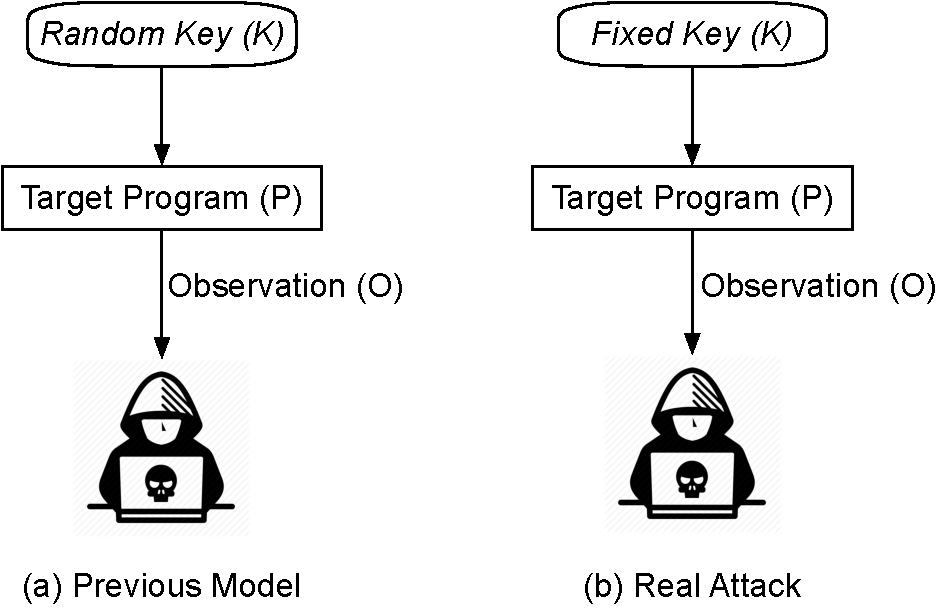
\includegraphics[width=.8\columnwidth]{./figures/RA.pdf}
   \caption{The gap between the real attack and previous model}
\end{figure}


\subsection{Notations}
In the section, we give the necessary definitions and notations for dealing 
with programs and side-channels. We use capital letters (e.g., $A$) to represent 
the set. $|S|$ represents the size of set $A$. We use corresponding small letters
to represents one element in the set (e.g., $a \in A$).

We assume the program ($\beta$) has $K$ as the sensitive input. 
$K$ should be a finite set of keys. The program also takes known messages $M$ as the input. 
The model applies to most of the cryptosystems. For example,
during the AES encryption, $\beta$ is the encryption function. $K$ is AES key and
$M$ is the message to be encrypted. During the execution, an adversary may have some observations ($O$) from the program. Examples of those observations
include timing, CPU usages, and Electromagnetic signals (EM). For this paper, we
consider the secret-dependent control-flows and secret-dependent memory accesses
as the observations.

With the above definitions, we have the following mapping between $\beta$, $K$, $M$, and $O$:

\begin{displaymath}
    \beta(K, M) \rightarrow O
\end{displaymath}

An adversary does not have access to $K$, but he knows $\beta$, $M$, and $O$. 
For one execution of a deterministic program, once $k \in K$ and $m \in M$ are fixed, the 
observation ($o \in O$) is also determined. As an attacker, he knows $\beta$, $o$, 
and $m$. The attacker wants to infer the value of $k$. We use $K^o$ to denote the set of
possible $k$ values that still produce the same observations:

\begin{displaymath}
    K^o = \{ k \in K \, |\, \beta(k, m) \rightarrow o\}
\end{displaymath}
Then the problem of quantifying the amount of leaked information can be transferred into the
following question. 
\emph{How much uncertainty of $K$ can be reduced if an attacker knows $\beta$, $m$, and $o$?}
 
\subsection{Theoretical Analysis}
Now we present our metric to quantify the amount of leaked 
information from dynamic analysis.

In information theory, the mutual information (MI) of is a measure of the mutual dependence 
between the two variables. Here we use MI to describe the leakage between $K$ and $O$, 
which is defined as:

\begin{equation} \label{eq:1}
    I(K;O) = \sum_{k {\in} K}{\sum_{o {\in} O}{p(k, o)\log_2\frac{p(k, o)}{p(k)p(o)}}}
\end{equation}

where $P(k_i, o_i)$ is the joint discrete distribution of $K$ and $O$.
Alternatively, the mutual information can also be equivalently expressed as:
\begin{equation} \label{eq:2}
    I(K;O) = H(K) - H(K|O)
\end{equation}

$H(K|O)$ is the entropy of $K$ conditioned on $O$. It quantifies the uncertainty of $K$
given the value of $O$. In other word, the conditional entropy $H(K|O)$ marks the 
uncertainty about $K$ after the adversary has gained some observations ($O$). 
\begin{equation}
    H(K|O) = - \sum_{o {\in} O} {p(o) \sum_{k {\in} K}{p(k|o)\log_2p(k|o)}}
\end{equation}

In the project, we hope to give a very precise definition of information leakages. 
Suppose an attacker run the target program multiple times with one fixed input, we
want to know how much information he can infer by observing the memory access patterns ($o$).
We come to the simple slogan ~\cite{10.1007/978-3-642-00596-1_21} %% where the information
%% leakage equals:
%% \textbf{Initial uncertainty - remaining uncertainty}
that
\begin{align*}
 & \mathit{Information\ leakage} = \\
 & ~~~~~~ \mathit{Initial\ uncertainty} - \mathit{Remaining\ uncertainty}. 
\end{align*}

Now we come compare the equation~\ref{eq:2} with the above slogan, we will
find $H(K)$ is the $\mathit{Initial\ uncertainty}$ and $H(K|O)$ is
$\mathit{Remaining\ uncertainty}$. During a side-channel attack, 
the observation ($o$) is known.  We have $H(K|O) = H(K|o)$.

Therefore, we define the amount of leaked information as 
\begin{displaymath}
    Leakage = H(K;o) = H(K) - H(K|o)
\end{displaymath}

For a program ($\beta$) without knowing any domain information, any sensitive
input should appear equally. Therefore, for any $k \in K$, $p(k) = \frac{1}{|K|}$.
So we have 
$$H(K) = \sum_{k {\in} K}\frac{1}{|K|}\log_2{|K|} = \log_2{|K|}$$
For any $k' \in K - K^o$, $p(k'|o) = 0$. We can get the following equation:
\begin{align*}
H(K;o) &= - \sum_{k {\in} K^o}{p(k|o)\log_2p(k|o)} 
          - \sum_{k` {\in} (K - K^o)}{p(k'|o)\log_2p(k'|o)}\\
       &= \sum_{k {\in} K^o}\frac{1}{|K^o|}\log_2{|K^o|}\\
       &= \log_2{|K^o|}
\end{align*}

\newtheorem{mydef}{Definition}

\begin{mydef}
\label{def}
Given a program $\beta$ with the input set $K$, 
an adversary has the observation $o$ when the input $k{\in}K^o$. 
We denote it as
$$\beta(K^o, m) \rightarrow	o$$

The leakage $L_{\beta(k)\rightarrow o}$ based on the observation ($o$) is
    $$L_{\beta(k)\rightarrow o} = \log_2{|K|} - \log_2{|K^o|}$$
\end{mydef}

With the new definition, if the attacker observes that the code~\ref{figure:password checker} runs the branch 1, 
then the $K^{o^{1}} = \{\mathrm{0x1b}\}$. Therefore, the information leakage $L_{P(k)=o^{1}} = \log_2{256} - \log_2{1} = 8$
bits, which means the key is totally leaked. If the attacker observes the code runs branch2, the leaked information is 
$L_{P(k)=o^{2}} = \log_2{256} - \log_2{255} = 0$ bit.


We can also calculate the leaked information
from the sample code~\ref{background::side-channel}. As the size of input 
sensitive information is usually public. The problem of quantifying the
leaked information has been transferred into the problem of estimating
the size of input key $|K^o|$ under the condition $o \in O$.

\begin{table}[ht]
    \centering

 %  \resizebox{.8\columnwidth}{!}{

\begin{tabular}{l|cccc}
    \hline
%Observation (o)     & $\emptyset$ & ${\{1\}}$ & ${\{2\}}$ & ${\{1, 2\}}$ \\ \hline
%Number of Solutions &  32876 & 20 & 32634 & 16 \\ \hline
%Possibility (p)     & 0.5016 & 0.0003 & 0.4980  & 0.0002   \\
Observation ($o$)  & $\emptyset$ & ${\{1\}}$ & ${\{2\}}$ & ${\{1, 2\}}$ \\ \hline
Number of Solutions &  32876 & 20 & 32634 & 16 \\ \hline
Leaked Information (bits)     & 1.0 & 11.7 & 1.0  & 12.0   \\
    \hline
\end{tabular}
%    }
\caption{The distribution of observations}
\label{shtable}
\end{table}

\subsection{Our Conceptual Framework}
We now discuss how we model the observation (o), which is the direct information
that an adversary can get during the attack.

During the execution, a program ($\beta$) have many temporary values ($t_i \in T$).
Once $\beta, k, m$ is determined,  $t_i$ is also fixed. Therefore, 
$ t_i = f_i(\beta, k, m)$.
$f_ i$ is a function that can uniquely map the one to one relation 
between $t_i$ and ($\beta$, $k$, $m$). 

In the paper, we consider two code patterns can be exploited by an attacker:
\emph{secret-dependent control transfers} and \emph{secret-dependent data accesses}.
In other words, an adversary have observations based on control-flows and
data accesses.

\subsubsection{Secret-dependent Control Transfers}
We think a control-flow is secret-dependence if different input sensitive keys ($K$)
can lead to different branch conditions. For a specific branch, the branch
condition is either true or false. Therefore, the branch condition is always a
boolean variable. 

We think a branch is secret-dependent if:
$$\exists k_{i1}, k_{i2} \in K, \,f_i(\beta, k_{i1}, m) \neq f_i(\beta, k_{i2}, m)$$

An adversary can observe which branch the code executes, if the branch condition
equals to $t_b$. We use the constraint $c_i : f_i(\beta, k, m) = t_b$ to model the
observation on secret-dependent control-transfers. 

\subsubsection{Secret-dependent Data Accesses}
Similar to secret-dependent control transfers, a data access is secret-dependence 
if different input sensitive keys ($K$) can lead to different memory addresses.
We use the model from~\cite{203878}. The low $L$ bits of the address is irrelevant
in side-channels. 

We think a data access is secret-dependent if:
$$\exists k_{i1}, k_{i2} \in K, \,f_i(\beta, k_{i1}, m) >> L \neq f_i(\beta, k_{i2}, m) >> L$$

If the branch condition equals to $t_b$,
we can use the constraint $c_i : f_i(\beta, k, m) >> L = t_b >> L$ to model the
observation on secret-dependent control-transfers. 

With the following definition, we can model an attacker's observation with math formulas.
For example~\ref{background::side-channel}, if an attacker observes
the code executes 1, we have $c_5: k_1 + k_2 < 8$ to describe an
attacker's knowledge and $K^{o5} = \{k_1,\, k_2\,|\, (k_1 + k_2) < 8\}$. If an attacker observes
the code executes 2, we have $c_8: k_1 - k_2 > 0$ 
and $K^{o8} = \{k_1,\, k_2\,|\, (k_1 - k_2) > 0\}$. 

\section{Scalable to Real-world Crypto Systems}
\label{sec:scala}

In \S\ref{sec:trace-qif}, we propose a better information leakage definition
for realistic attack scenarios, model two types of address-based side-channel
leakages
as math formulas, and quantify them by calculating the number of input
keys ($K^o$) that satisfy those math formulas. Intuitively, we can use
traditional symbolic execution to capture math formulas and use model
counting to get the number of satisfying input keys ($K^o$).
However, some preliminary experiments show that above approach suffers from the unbearable cost,
which impede its usage
to detect and quantify side-channel leakages in real-world applications.
In this section, we begin by discussing the bottlenecks of applying the
above approaches in real-world crypto systems. After that, we propose
our methods.

In general, \tool{} faces the following performance and cost  challenges
in order to \emph{scale to production crypto system analysis}.
\begin{itemize}
      \item Symbolic execution (\textbf{Challenge C2})
      \item Constraint solving (\textbf{Challenge C3})
      \item Counting the number of items in $K^o$ (\textbf{Challenge C4})
\end{itemize}

\subsection{Trace-oriented Symbolic Execution}
While symbolic execution can capture the fine-grained semantics of programs,
it is also notorious for its unbearable performance cost. Previous
trace-oriented symbolic execution based
works~\cite{203878,Chattopadhyay:2017:QIL:3127041.3127044} all
have large performance bottlenecks. As a result, those approaches
either only apply to small-size programs~\cite{Chattopadhyay:2017:QIL:3127041.3127044}
or apply some domain knowledge to simplify the analysis.
Those tools interpret each instruction and update the memory cells and registers with
formulas that captured the semantics of the execution and search different
input values that can lead to different execution behaviors using constraint solver.
We implement the approach presented in \S\ref{sec:trace-qif} and
model the side-channels as formulas.
While the tool can finish analyzing some simple cases like AES,
it can not handle complicated cases like RSA.

We observe that finding side-channels using symbolic execution is different from
traditional general symbolic execution and can be optimized to be as efficient as other
methods with the approaches  below.

%\subsubsection{Interpret Instructions Symbolically}

The number of machine instructions is enormous, and the semantics of each instruction is complex.
Intel Developer Manual~\cite{intelsys}
introduces more than 1000 different x86 instructions.
It is tedious to implement the manual
rules for every instruction.

Therefore, existing binary analysis tools~\cite{shoshitaishvili2016state, 10.1007/978-3-642-22110-1_37}
usually translate machine instructions into intermediate languages (IR).
The IR typically has fewer instructions compared to the original machine ISA\@.
However, the IR layer designs, which significantly
simplify the implementation, also introduce significant overhead~\cite{217563}.
First, transferring machine
instruction into IR is time-consuming.
For example, REIL IR~\cite{dullien2009reil}, adopted in
CacheS~\cite{236338}, has multiple transform processes, from binary to VEX IR, BAP IR,
and finally REIL IR\@.
As IR can also introduce additional conditional jump instructions,
in order to precisely identify secret-dependent control-flow,
we need to rule out conditional jump instructions introduced by
IR, which is also time-consuming. Second, IR increases the total
number of instructions. For example, x86 instruction \textit{test eax, eax}
transfers into 18 REIL IR instructions. If we assume the time of symbolically executing
one instruction is constant, the design of adopting IR layers can introduce large overhead.

\vspace*{2pt}
\textbf{Our Solution to Challenge C2:}
We adopt the approach from~\cite{217563} and implement the symbolic execution
directly on the top x86 instructions. Table~\ref{scala:ir}
shows that eliminating the IR layer can reduce the number
of instructions executed during the analysis.

\begin{table}%[ht]
      \centering%\small\footnotesize
      \caption{The number of x86 instructions and the number
            of REIL and VEX IR instructions on each trace of crypto programs.}
      \label{scala:ir}
      \resizebox{\columnwidth}{!}{%

            \begin{tabular}{cccc}
                  \hline
                                    & \begin{tabular}[c]{@{}c@{}}Number of\\ x86 Instructions\end{tabular} & \begin{tabular}[c]{@{}c@{}}Number of\\ VEX IR\end{tabular} & \begin{tabular}[c]{@{}c@{}}Number of\\ REIL IR\end{tabular} \\ \hline
                  AES OpenSSL 0.9.7 & $1,704$                   & $23,938$ (15x)            & $62,045$ (36x)            \\
                  DES OpenSSL 0.9.7 & $2,976$                   & $41,897$ (15x)            & $100,365$ (33x)           \\
                  RSA OpenSSL 0.9.7 & $1.6*10^7$                & $2.4*10^8$ (15x)          & $5.9*10^8$ (37x)          \\
                  RSA mbed TLS 2.5  & $2.2*10^7$                & $3.1*10^8$ (15x)          & $8.6*10^8$  (39x)         \\ \hline
            \end{tabular}
      }
\end{table}

\subsection{Constraint Solving}
As discussed in \S\ref{side-channel:condition}, the problem
of identifying side-channels can be reduced to the
question below.

\begin{quote}
      \textit{Can we find two different input variables $k_1, k_2 \in K$ that satisfy the
            formula $f_a(k_1) \neq f_a(k_2)$?}
\end{quote}

Existing approach relies on satisfiability modulo theories (SMT) solvers (e.g, Z3) to
find satisfying $k_1$ and $k_2$.
We argue that while it is a universal approach to solving constraints with SMT
solvers, for constraints with the above formats, using custom heuristics and testing
is much more
efficient in practice. Constraint solving is a decision problem expressed in
logic formulas. SMT solvers transfer the inputted SMT formula into
the boolean conjunctive normal form (CNF) and feed it into the internal
SAT solver. The translation process, called ``bit blasting'', is time-consuming.
Also, as SAT problem is a well-known NP-complete problem, it is also hard to
deal when it comes to practical uses with very large formulas.
Despite the rapid development of SMT solvers in recent years, constraint solving still
remains one of the obstacles to achieve the scalability for real-world crypto systems.

\vspace*{2pt}
\textbf{Our Solution to Challenge C3:}
Instead of feeding the formula $f_a(k_1) \neq f_a(k_2)$ into a SMT solver, we just
randomly pick up $k_1, k_2 \in K$ and test them if they can satisfy the formula. Our
solution is based on the following intuition. For most combination of
$(k_{1}, k_{2} )$, the formula $f_a(k_1) \neq f_a(k_2)$ holds. As long as
$f_a$ is not a constant function, such $k_1, k_2$ must exist. For example,
suppose each time we only have 5\% chance to find such $k_1, k_2$, then
after we test with different input combination with 100 times, we have
$1 - (1-0.05)^{100} = 99.6\%$ chance find such $k_1, k_2$. Such random algorithms
work well for our problem.

\subsection{Counting the Number}
\label{MCreasons}
The problem of quantifying the amount of leaked information can be reduced to
the problem of computing the number of items in $K^o$, according to Definition~\ref{def}
introduced in \S\ref{sec:trace-qif}.
However, we find while there are various propositional model counters (e.g., \#SAT),
they are not sufficient scalable for production crypto system analysis.
%there is no open source modulo theories counter (\#SMT) available.

One naive method approximating the number of solutions is based on Monte Carlo sampling.
However, the number of satisfying values could be exponentially small. Consider the formula
$f_i\equiv{k_1} = 1\land{k_2} = 2\land{k_3} = 3\land{k_4} = 4$, where $k_1$, $k_2$, $k_3$, and $k_4$ each represents one byte in the original sensitive input buffer,
there is only one satisfying solution of total $2^{32}$ possible
values, which requires exponentially many samples to get a tight bound.
Monte Carlo method also suffers from the curse of dimensionality. For example,
the length of RSA private key can be as long as 4096 bits.
If we take each byte (8 bits) in the original buffer as one symbol, the formula can have
as many as 512 symbols.

\vspace*{6pt}
\textbf{Our Solution to Challenge C4:}
We adopt multiple step Monte Carlo sampling methods to count the number of possible inputs
that satisfy the logic formula groups. The key idea is to
split those constraints into several small formulas and sample them independently.
%We will introduce the method in the following subsection.

\subsection{Information Leakage Estimation}

\newcommand{\addr}[1]{{l}_{#1}}
\renewcommand{\addr}[1]{{\gamma}_{#1}}
\renewcommand{\addr}[1]{{\zeta}_{#1}}
\renewcommand{\addr}[1]{{\xi}_{#1}}

In this section, we present the algorithm to calculate the information
leakage based on Definition~\ref{def} (\S\ref{sec:trace-qif}), answering to
\textbf{Challenge C4}.

\subsubsection{Problem Statement}
With each leakage site, we model it with a math formula constraint with the method
presented in~\S\ref{side-channel:condition}.
Suppose the address of the leakage site is $\addr{i}$,
we use $c_{\addr{i}}$ to denote the constraint. For multiple leakage sites,
we use the conjunction of those constraints to represent those leakage sites.

According to the definition~\ref{def}, to calculate the amount of leaked
information, the key is calculating $\frac{|K|}{|K^o|}$. $K^o$ represents
the set that contains every input keys that satisfy the constraint. As the
cardinality of $K$ is known, the key problem is to estimate the cardinality of
$K^o$. Suppose an attacker can observe $n$ leakage sites, and each leakage site has
the following constraints: $c_{\addr{1}}, c_{\addr{2}}, \ldots, c_{\addr{n}}$ respectively.
The total leakage has the constraint
$c_t({\addr{1}},{\addr{2}},\ldots,{\addr{n}}) = c_{\addr{1}} \land c_{\addr{2}}
      \land \ldots \land c_{\addr{n}}$. The problem of estimating the total leaked information
can be reduced to the problem of counting the number of different solutions
that satisfies the constraint $c_t({\addr{1}},{\addr{2}},\ldots,{\addr{n}})$.
A native method for approximating
the result is to pick $k$ elements from $K$ and check how many of them are also
contained in $K^o$. If $q$ elements are also in $K^o$. In expectation, we can
use $\frac{k}{q}$ to approximate the value of $\frac{|K|}{|K^o|}$.

However, as discussed in \S\ref{MCreasons},
the above sampling method will typically fail in practice due to the following two problems:

\begin{enumerate}
      \item The curse of dimensionality. $c_t({\addr{1}},\ldots,{\addr{n}})$ is
            the conjunction of many constraints.
            Therefore, the input variables of each constraints will also be
            the input variables of the $c_t({\addr{1}},\ldots,{\addr{n}})$.
            The sampling method will fail as
            $n$ increases. For example, if the program has $2$ byte input equals to 2,
            the whole search space is
            a $256^2$ cube. If we want the sampling distance between each point equals to $d$,
            we need $256^2d$ points. If the program has $10$ byte input,
            we need $256^{10}d$ points if we
            still we want the sampling distance equals to $d$.

      \item The number of satisfying assignments could be exponentially small.
            According to Chernoff bound, we need exponentially many samples to get
            a tight bound. On an extreme situation, if the constraint only has one unique
            satisfying solution, the simple Monte Carlo method cannot find the satisfying
            assignment even after sampling many points.
\end{enumerate}

However, despite the two problems. We also observe two characteristics
of the problem:
\begin{enumerate}
      \item $c_t({\addr{1}},{\addr{2}},\ldots,{\addr{n}})$ is the conjunction of several
            short constraints $c_{\addr{i}}$. The set containing the input variables of
            $c_{\addr{i}}$ is the subset of the input variables of
            $c_t({\addr{1}},{\addr{2}},\ldots,{\addr{n}})$.
            Some constraints have completely different input variables from other constraints.
            %\item For each constraint $F(C_{{addr}_i})$, the satisfying assignments
            %are close to each other, which means if we find one satisfying assignment, we 
            %are more likely to find other satisfying assignments nearby than randomly
            %pick one point in the whole searching space.

\end{enumerate}

In regard to the above problems, we present our methods. First, we split
$c_t(\addr{1},\addr{2},\ldots,\addr{n})$ into several independent constraint groups. After
that, we run multiple step sampling method for each constraint.

\subsubsection{Maximum Independent Partition}

For a constraint $c_{\addr{i}}$, we define function $\pi$, which maps
the constraint into a set of different input symbols. For example,
$\pi(k1 + k2 > 128) = \{k1, k2\}$.

\begin{mydef}[]
      \label{independentC}
      Given two constraints $c_m$ and $c_n$, we call them independent iff
      $$\pi(c_m) \cap \pi(c_n) = \emptyset$$
\end{mydef}

Based on the definition~\ref{independentC}, we can split
the constraint $c_t(\addr{1},\addr{2},\ldots,\addr{n})$ into several
independent constraints. There are many partitions. For our project,
we are interested in the following one.

\begin{mydef}\label{Goodpartition}
      For the constraint $c_t(\addr{1},\addr{2},\ldots,\addr{n})$,
      we call the constraint group
      $g_{1}, g_{2}, \ldots, g_{m}$
      the maximum independent partition of $c_t(\addr{1},\addr{2},\ldots,\addr{n})$ iff
      \begin{enumerate}
            \item $g_{1} \land g_{2} \land \ldots \land g_{m} = c_t(\addr{1},\addr{2},\ldots,\addr{n})$
            \item $\forall \quad i, j \in \{1, 2, 3, \ldots, m\} \quad \textrm{and} \quad
                        i \neq j, \quad \pi(g_{i}) \cap \pi(g_{j}) = \emptyset $
            \item For any other partitions  $h_{1}, h_{2}, \ldots, h_{m'}$ satisfy 1) and
                  2), $m \geq m'$
      \end{enumerate}

\end{mydef}

The reason we want a good partition of the constraints is that we want to
reduce the dimensions. Consider the example in the previous section,
$$c: ({k_1} = 1)\land({k_2} = 2)\land({k_3} > 4)\land({k_3} - {k_4} > 10)$$
A good partition of $F$ would be
$$g_{1}: ({k_1} = 1)\quad g_{2}: ({k_2} = 2)\quad g_{3}: ({k_3} > 4) \land ({k_3} - {k_4} > 10)$$
So instead of sampling in the four dimension space, we can
sample each constraint in the less dimension space and combine them
together with Theorem~\ref{IndependentConstraint} .

\begin{theorem}
      \label{IndependentConstraint}
      Let $g_{1}, g_{2}, \ldots, g_{m}$ be a maximum independent partition of
      $c_t(\addr{1},\addr{2},\ldots,\addr{n})$.
      $K_c$ is the input set that satisfies constraint $c$. We can have the following
      equation in regard to the size of $K_c$
      $$|K_{c_t(\addr{1},\addr{2},\ldots,\addr{n})}| = |K_{g_{1}}|*|K_{g_{2}}|*\ldots*|K_{g_{n}}|$$
\end{theorem}

With Theorem~\ref{IndependentConstraint}, we can transfer the problem of counting the number of
solutions in a large constraint with high
dimensions into counting solutions of
several small constraints. We apply the following algorithm~\ref{algo:max-inde} to get the
Maximum Independent Partition
of the $c_t(\addr{1},\addr{2},\ldots,\addr{n})$.

\IncMargin{1em}
\begin{algorithm}[h]
      \DontPrintSemicolon
      \SetKwInOut{Input}{input}\SetKwInOut{Output}{output}
      \Input{$c_t(\addr{1},\addr{2},\ldots,\addr{n}) = c_{\addr{1}} \land c_{\addr{2}} \land \ldots \land c_{\addr{m}}$}
      \Output{The Maximum Independent Partition of $G = \{g_{1}, g_{2}  , \ldots,  g_{m} \}$ }
      \For{$i\leftarrow 1$ \KwTo $n$}
      {
            $S_{c_i}$ $\leftarrow$ $\pi(c_{\addr{i}})$ \;
            \For{$g_{i} \in G$}
            {
                  $S_{g_i}$ $\leftarrow$ $\pi(g_{i})$ \;
                  $S$ $\leftarrow$ $S_{C_i} \cap S_{G_i}$  \;
                  \If{$S \neq \emptyset$}
                  {
                        $g_{i} \leftarrow g_{i} \land g_{\addr{i}}$ \;
                        \textbf{break} \;
                  }
                  Insert $c_{\addr{i}}$ to $G$
            }
      }
      \caption{The Maximum Independent Partition}
      \label{algo:max-inde}
\end{algorithm}
\DecMargin{1em}

\subsubsection{Multiple Step Monte Carlo Sampling}

After we split those constraints into several small constraints, we count
the number of solutions for each constraint. Even though the dimension
has been reduced greatly after the previous step, this is still a
\#P problem. For our project, we apply the approximate counting instead of
exact counting for two reasons. First, we don't need to have a very precise
result of the exact number of total solutions. As the information is defined with
a logarithmic function. We do not need to distinguish between constraints having
$10^{10}$ or $10^{10} + 10$ solutions.
Second, as the constraint could be very complicated. The exact model counting
approaches, like DPLL search, have difficulty scaling up to large problem sizes.

We apply the ``counting by sampling" method. The basic idea is as follows.
For the constraint $g_{i}= c_{i_1} \land c_{i_2} \land ,\ldots, \land c_{i_j} \land ,\ldots,
      \land c_{i_m}$,
if the solution satisfies $g_{i}$, it should also
satisfies any constraint from $c_{i_1}$ to $c_{i_m}$. In other words,
$K_{c_gi}$ should be the subset of $K_{c_1}$, $K_{c_2}$, \ldots , $K_{c_m}$.
We notice that $c_i$ usually has less numbers of input compared to $g_{i}$.
For example, if $c_{i_j}$ has only one input variable, we can find the exact
solution set $K_{c_{i_j}}$ of $c_{i_j}$ by trying every possible 256 solutions. After that,
we can only generate random input numbers for the rest input variables in
constraint $g_{i}$. With the simple trick, we can reduce the number of input while
still ensure the accuracy.

%% the algorithm
%\IncMargin{1em}
%\begin{algorithm}
%\SetAlgoLined
%\DontPrintSemicolon

%\KwIn{{The constraint $G_{i}= C_{i_1} \land C_{i_2}
%\land \ldots \land C_{i_m}$}}    
%\KwOut{{The number of assignments that satisfy $G_{i}$ $|K_{G_{i}}|$}}

%\SetKwProg{RW}{RandomWalk}{}{}
%\SetKwProg{MM}{MetropolisMove}{}{} 
%$n$: the number of sampling times \;
%$P$: a probability generator \;
%$k$: the input assignment \;
%$n_{s}$: the number of satisfying assignments \;
%$\#k$: the satisfying number of k \fixme{this number is not used syntactically} \; 
%Initialization: \;
%$\#{k_0}$ $\leftarrow$ $\sum_{j=1}^{m}C_{i_j}(k_0)$ \;
%\For{$t\leftarrow 1$ \KwTo $n$} {
%      $p$ $\leftarrow$ $P$ \;
%      \If{$p \geq 0.5$}
%      {
%        $v$ $\leftarrow$ \RW{$v$} {}
%      }
%      \Else{
%            $v$ $\leftarrow$ \MM{$v$} {}
%      }
%      \If{$v$ satisfies $G_{i}$}
%      {$n_{s}$ $\leftarrow$ $n_{s} + 1$}
%}
%$|K_{G_{i}}|$ $\leftarrow$ $n_s|K| / n$
%\caption{Metropolis Sampling}
%\end{algorithm}
%\DecMargin{1em}

\subsubsection{Error Estimation}
In this part, we analyze the accuracy the result from Monte Carlo approximation.
We use central limit theorem (CLT) and uncertainty propagation theorem
to estimate errors of the number of leaked bits for each site.

Let $n$ be the number of samples and $n_s$ be the number of samples
that satisfy the constraint $C$. Then we can get $\hat{p} = \frac{n_s}{n}$.
If we run the same experiment multiple times, each time we can
get a $\hat{p}$.
As each $\hat{p}$ is independent and identically distributed, according to
central limit theorem, the mean value should
satisfy normal distribution.
$$ \frac{\bar{p}-E(p)}{\sigma\sqrt{n}} \rightarrow N(0,1) $$
Here $E(p)$ is the mean value of $p$ and $\sigma$ is the standard
variance of $p$. If we use the observed value $\hat{p}$
to the represent standard deviation.
We can claim that we have 95\% confidence that the error
$\Delta p= \bar{p} - E(p)$ falls in the interval:
$$ |\Delta p| \leq 1.96\sqrt{\frac{ \hat{p} (1- \hat{p} )}{n}}$$

Since we use $L = \log_{2}p$ to estimate the amount of leaked information,
we can have the following error propagation formula $\Delta L = \frac{\Delta p}{p\ln2}$
by differentiation. For \tool, we want the error of estimated leaked information ($\Delta L$) is
less than 1 bit. So we can get $\frac{\Delta p}{p\ln2} \leq 1$. As long as
$ n \geq \frac{1.96^2(1-p)}{p(\ln2)^2}$, we have 95\% confidence the error of estimated
leaked information is less than 1 bit. During the simulation, if $n$ and $p$ satisfy
the above equation, Monte Carlo Simulation will terminate.




\section{Design}
In this section, we describe the design of \tool{} by focusing on
how our design solves the three challenges discussed in the previous
section.

\subsection{Trace Logging}
The trace information can be logged via some emulators (e.g., QEMU) or 
dynamic binary instrumentation tools (DBI). 
We run a program with the concrete input under the DBI to record the
execution trace.
The trace data has the following information:
\begin{itemize}
    \item Each instruction mnemonics and its memory address.
    \item The operands of each instruction and their concrete values during the 
          runtime.
    \item The value of eflags register. 
    \item The memory address and the length of the sensitive information.
     Most software developers stores sensitive information in an array,
     a variable or a buffer, which means that those data is stored in a contiguous 
     area in the memory. We use the symbol information in the binary to track the 
     address in the memory.
\end{itemize}

\subsection{Instruction Level Symbolic Execution}
\label{InstructionSE}
The main purpose of the step is to generate 
constraints of the input sensitive information from the execution trace. 
If we give the target program a new input which 
is different from the origin input that was used 
to generate the execution trace but still satisfies those constraints,
the new execution trace still have the same control flow and 
data access patterns. 

The tool runs the symbolic execution on the top of the execution traces.
At the beginning of the symbolic execution, the tool creates fresh 
symbols for each byte in the sensitive buffer. For other data in the 
register or memory at the beginning, we use concrete values from the 
runtime information collected in
the previous step. During the symbolic execution for each instruction, 
the tool updates every variable in the memory and registers with a
math formula. The formula is made up with concrete values and 
the input key as the symbols accumulated through the symbolic execution.
For each formula, the tool will check weather it can be reduced
into a concrete values (e.g., $k_1+12-k_1 = 12$ ). 
If so, the tool will only use the concrete values in the 
following symbolic execution.

\subsubsection{Verification and Optimization}
We run the symbolic execution(SE) on the top of x86 instructions.
In other words, we don’t rely on any intermediate languages to 
simplify the implemetation of symbolic execution. 
While the implementation itself 
has a lot of benefits (Better performance, accurate memory model), 
we need to implement the symbolic execution 
rules for each X86 instruction. 
However, due to the complexity of X86, it is inevitable to make mistakes. 
Therefore, we verify the correctness of the SE engine during the execution. 
The tool will collect the runtime information (Register values, 
memory values) and compare them with the formula generated from the 
symbolic execution. Whenever the tool finishes the symbolic execution 
of each instruction, the tool will compare the formula for each symbol 
and its actual value. If the two values don't match, we check the code
and fix the error. Also, if the formula doesn't contain any symbols,
the tool will use the concrete value instead of symbolic execution.

\subsubsection{Secret-dependent control-flows}
An adversary can infer sensitive information from secret dependent control-flows. 
There are two kinds of control-transfer instructions: the unconditional 
control-transfer instructions and the conditional transfer instructions.
The unconditional instructions, like CALL, JUMP, RET transfer control
from one code segment location to another. Since the transfer is 
independent from the input sensitive information, an attacker was 
not able to infer any sensitive information from the control-flow. 
So the unconditional control-transfer doesn't leak any information 
based on our threat model. During the symbolic execution, 
we just update the register information and memory cells with 
new formulas accordingly.

The conditional control-flow transfer instructions, like conditional jumps,
depending on CPU states, may or may not transfer control flows.
For conditional jumps, the CPU will test if certain condition flag 
(e.g., CF = 0, ZF =1) is met and jump to the certain branches respectively.
The symbolic engine will compute the flag and represent the flag 
in a symbol formula. Because we are running on a symbolic execution 
on a execution trace, we know which branch is executed.
If a conditional jump uses the CPU status flag, we will generate 
the constraint accordingly.

\begin{figure}[ht]
      \centering
      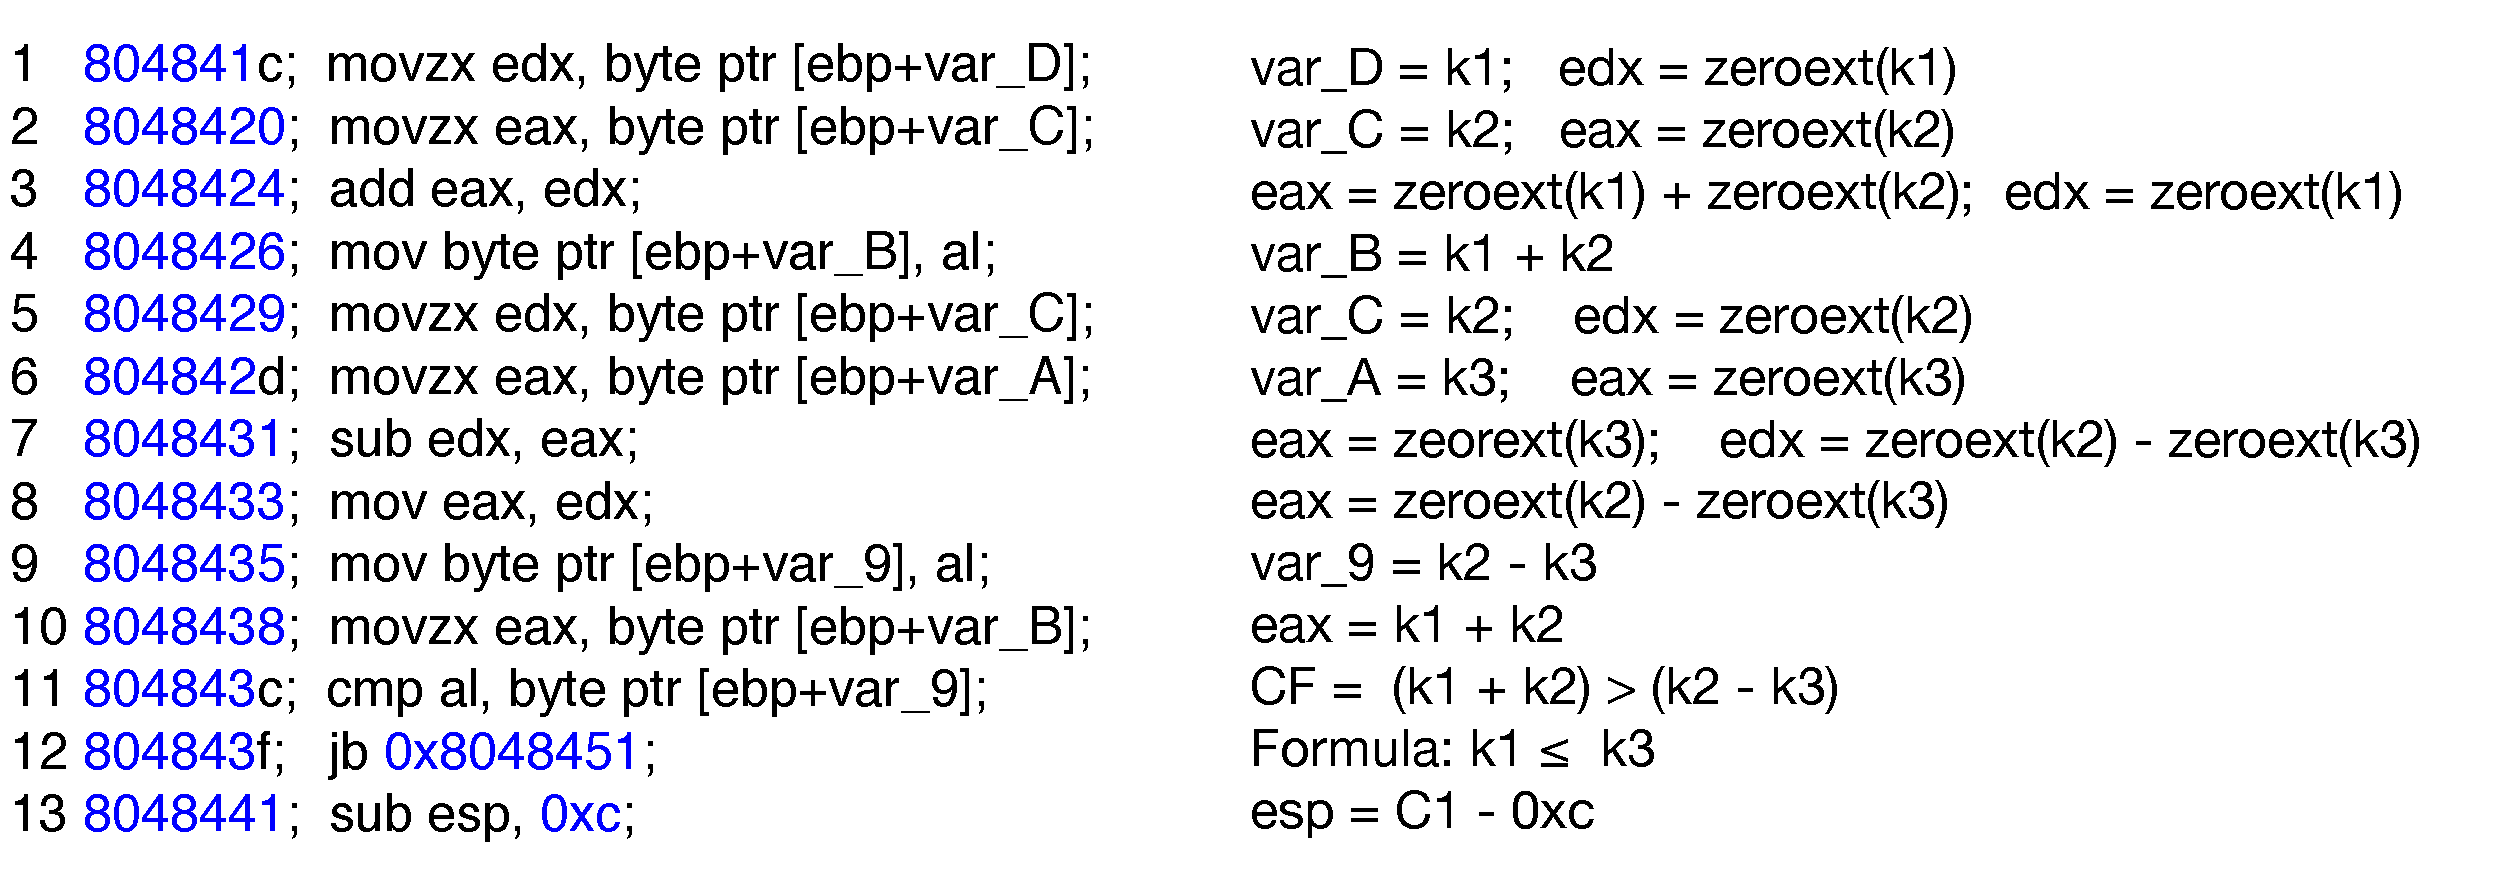
\includegraphics[width=\columnwidth]{./figures/secretCF.pdf}
      \caption{The workflow of \tool{}}
      \label{fig:Test}
  \end{figure}

For examples,

\begin{lstlisting}
...
0x0000e781      add dword [local_14h], 1
0x0000e785      cmp dword [local_14h], 4
0x0000e789      jne 0xe7df
0x0000e78b      mov dword [local_14h], 0
...
\end{lstlisting}

At the beginning of the instruction segment, the value at the 
address of local14h can be written as $F(\vec{K})$. At the address e785, 
the value will be updated with $F(\vec{K})+1$. Then the code compares 
the value with 4 and use the result as a conditional jump. 
Based on the result, we can have the following formula:

$$F(\vec{K}) + 1 = 4$$

The formula, together with the memory address (0xe789) is store
as a \textit{formula tuple (address, formula)}. 
Each formula tuple represents one leakage site.

\subsubsection{Secret-dependent data access}
Like input-dependent control-flow transfers, an adversary can also infer 
sensitive information from the data access pattern as well. 
We try to find this kind of leakages by checking 
every memory operand of the instruction. We generate the memory addressing 
formulas. As discussed before, every symbols in the formula is the input key. 
If the formula doesn’t contain any symbols, the memory access is independent 
from the input sensitive information and won’t leak any sensitive information 
according to our threat model. Otherwise, we will generate the constraint for
the memory addressing. We model the memory address with a symbolic formula 
$F(\vec{K})$. 
Because we also have the concrete value of the memory address $Addr1$. Therefore,
the formula can be written as:

$$F(\vec{K}) = Addr1$$

\subsection{Markov Chain Monte Carlo Approximate Counting}

From the above step~\ref{InstructionSE}, we can generate the constraints 
from the execution trace. 
The only variables in those constraints are the sensitive data. An adversary who 
wants to infer the sensitive data based on side-channel attacks can't observe 
the sensitive information directly. The adversary, however, can observe the
memory access pattern of the software. Each math formula can uniquely model
one leakage site.

In this section, we calculate the amount of leaked information with the
definition from~\ref{def}. The basic idea is to calculate $\frac{|K|}{|K^o|}$.
The size of $K$ is usually exponentially large. A naive method for approximating
the result is to pick $k$ elements from $K$ and check how many of them are also
contained in $K^o$. If $q$ elements are also in $K^o$. In expectation, we can
use $\frac{k}{q}$ to approximate the value of $\frac{|K|}{|K^o|}$. In this step,
we first split the contrains tuple into multiple groups depending on the memory
address. After that, we run the Markov Chain Monte Carlo to estimate the amount
of leaked information.


\subsubsection{Preprocessing}
We apply two preprocessing steps before running the Monte Carlo sampling. First,
we try to simplify those formulas by applying some normalizations rules. After
that, we split those formulas into multiple groups.

The goal of the normalization is to simplify the formulas. 
Each formulas will be evaluated multiple times with different input 
during the following sampling, 
we would like to make those formula simpler to reduce the whole execution time.  
Each formula is implemented as a abstract syntax tree. We apply a series of 
normalization rules (e.g. key1 xor key1 = 0) to simplify the formula.

After that, we split the formula tuple into multiple groups. 
Each group consists of different formulas but with the same memory address.
In other words, those formulas in the same group represent one leakage
site. The instructions inside a loop are executed multiple times with
the different item from the input buffer. We group them together to 
know the total information leakage.

The only symbol in the original formula is the key. 
An adversary who wants to infer the sensitive data based on side-channel 
attacks can't observe the sensitive information directly. 

\subsubsection{Motivation}
The adversary, however, can observe the memory access pattern of the software. 
If the attacker can observe one leakage site, the attack is modeled as one formula. 
If he observes mutiple information leakage, the attack is modeled as the conjoint 
of those formulas. Calculating the total information leakage can be reduced to the
problem of approximating the number of solutions. This is a \#P problem.

One intuition way is to use the Monte Carlo method. However, 
as the discussion in the previous section~\ref{MCreasons},
the number of satisfying keys could be exponentially small. Imagine an attacker 
who can recover one unique key after the attack, in such case, 
the conjoint of formula F = (f(k)) only has one solution.
Also, the target program may have mutiple inputs. When the number of input
symbols arises, the simple Monte Carlo may suffer from the curse of dimensionality,
which means the accuracy of the result drops dramatically when the
number of input symbols increases. 

We adopt the Markov Chain Monte Carlo (MCMC) to estimate the number of 
satisfying solutions. The basic idea is to construct a Markov Chain that
has the desired distribution.

\textit{Definition:}
Starting from here, we present the formal definition of the MCMC algorithm.
First, we introduce the definition of the concept of the algorithm.

\begin{mydef}
      An approximation scheme is an alogorithm for finding an approximation
      answer within a factor $1 + \epsilon$ of the correct number of the set
      $K^o$ with the probability of $1 - \zeta$.
\end{mydef}

\newtheorem{theorem}{Theorem}[section]

\begin{theorem}
      If $F={A_1,A_2,...,A_n}$ is a finite collection of closed sets then 
      $\cup_{i}^{n}A_i$ is a closed set.
\end{theorem}

\subsubsection{MCMC Algorithm}
In the section, we present the detail of MCMC algorithm for counting the 
cardinality of $K^o$. We will fisrt present the description of the 
MCMC and then explain the algorithm with a concrete example.
\begin{enumerate}
      \item Start with the concrete input $\vec{k} = (k_0, k_1, k_2, ..., k_n)$,
      $\vec{k}$ should be the on valid solution which satisfies the constraint
      $F = C_1(\vec{k})\land C_2(\vec{k})\land C_2(\vec{k}) \land ... \land C_m(\vec{k})$
      \item for t = 1, 2, 3,..., N
\end{enumerate}
\section{Implementation}
We implement the \tana\ with 12K lines of code in C++11. It has three components, one Intel
Pin tool that can collect the execution trace, the intruction-level symbolic execution
engine and the backend that can estimate the information leakage. 

\section{Evaluation}
\label{res_overview}

\begin{table*}
    \centering
    \caption{Evaluation results overview. We evaluate two versions of mbedTLS and five
        versions of OpenSSL\@. CF represents secret-dependent control-flow transfers and
        DF represents secret-dependent data-flow transfers. Side-channel leakages can
        be found by symbolic execution and we run Monte Carlo to estimate the amount
        of leakage information. A summary of all vulnerabilities with the amount of
        leak information can be found in the appendix.
    }\label{table:over_result}
    \newlength{\x}
    \newlength{\y}
    \settowidth{\x}{~~}
    \settowidth{\y}{m}
    \addtolength{\x}{-1\y}
    \newcommand{\foo}{\mbox{\hspace*{\the\x}}}
    \begin{tabular}{clrrrrrrr}
        \hline
        \textbf{Algorithm} & \textbf{Implementation}  & \textbf{Leakage Sites} & \textbf{CF}         & \textbf{DF}
                           & \textbf{\# Instructions} & \textbf{Max Leakage}   & \textbf{Sym.\ Exe.} & \textbf{Monte Carlo}                                                    \\\hline
                           &                          &                        &                     &                      &             & bits & ms        & ms              \\\cline{7-9}
        AES                & Mbed TLS 2.5             & 68                     & 0                   & 68                   & 39,855      & 8.6  & 512 ~~    & 1,052 ~~        \\
        AES                & Mbed TLS 2.15            & 68                     & 0                   & 68                   & 39,855      & 9.1  & 520 ~~    & 1,057 ~~        \\
        AES                & OpenSSL 0.9.7            & 75                     & 0                   & 75                   & 1,704       & 10.6 & 231 ~~    & 9,199 ~~        \\
        AES                & OpenSSL 1.0.2f           & 88                     & 0                   & 88                   & 1,350       & 12.0 & 36 ~~     & 1,924 ~~        \\
        AES                & OpenSSL 1.0.2k           & 88                     & 0                   & 88                   & 1,350       & 12.5 & 35 ~~     & 1,961 ~~        \\
        AES                & OpenSSL 1.1.0f           & 88                     & 0                   & 88                   & 1,420       & 12.6 & 36 ~~     & 2,161 ~~        \\
        AES                & OpenSSL 1.1.1            & 88                     & 0                   & 88                   & 1,586       & 4.4  & 43 ~~     & 1,631 ~~        \\
        DES                & Mbed TLS 2.5             & 15                     & 0                   & 15                   & 4,596       & 1.1  & 58 ~~     & 162 ~~          \\
        DES                & Mbed TLS 2.15            & 15                     & 0                   & 15                   & 4,596       & 1.0  & 57 ~~     & 162 ~~          \\
        DES                & OpenSSL 0.9.7            & 6                      & 0                   & 6                    & 2,976       & 7.6  & 163 ~~    & 4,677       ~~  \\
        DES                & OpenSSL 1.0.2f           & 8                      & 0                   & 8                    & 2,593       & 9.8  & 166 ~~    & 6,509       ~~  \\
        DES                & OpenSSL 1.0.2k           & 8                      & 0                   & 8                    & 2,593       & 10.1 & 165 ~~    & 5,975        ~~ \\
        DES                & OpenSSL 1.1.0f           & 8                      & 0                   & 8                    & 4,260       & 8.8  & 182 ~~    & 5,292        ~~ \\
        DES                & OpenSSL 1.1.1            & 6                      & 0                   & 6                    & 8,272       & 7.5  & 229 ~~    & 5,152       ~~  \\
                           &                          &                        &                     &                      &             &      & minutes   & minutes         \\\cline{8-9}
        RSA                & Mbed TLS 2.5             & 6                      & 6                   & 0                    & 22,109,246  & 9.6  & 39 ~~     & 41  ~~          \\
        RSA                & Mbed TLS 2.15            & 12                     & 12                  & 0                    & 24,484,441  & 8.7  & 44 ~~     & 251  ~~         \\
        RSA                & OpenSSL 0.9.7            & 107                    & 105                 & 2                    & 17,002,523  & 17.2 & 23 ~~     & 428 ~~          \\
        RSA                & OpenSSL 1.0.2f           & 38                     & 27                  & 11                   & 14,468,307  & 16.2 & 29 ~~     & 436  ~~         \\
        RSA                & OpenSSL 1.0.2k           & 36                     & 27                  & 9                    & 15,285,210  & 14.2 & 40 ~~     & 714   ~~        \\
        RSA                & OpenSSL 1.1.0f           & 31                     & 22                  & 9                    & 16,390,750  & 17.2 & 34 ~~     & 490 ~~          \\
        RSA                & OpenSSL 1.1.1            & 27                     & 20                  & 7                    & 18,207,020  & 14.9 & 7 ~~      & 501 ~~          \\\hline
        Total              &                          & 886                    & 219                 & 667                  & 128,061,910 &      & 209m \foo & 2,861m \foo     \\\hline
        %                    &                          &                       &                     &                      &             & bits & ms        & ms              \\\cline{7-9}
        % AES                & Mbed TLS 2.5             & 68                    & 0                   & 68                   & 39,855      & 8    & 570 ~~    & 850 ~~          \\
        % AES                & Mbed TLS 2.15            & 68                    & 0                   & 68                   & 39,855      & 8    & 550 ~~    & 829 ~~          \\
        % AES                & OpenSSL 0.9.7            & 75                    & 0                   & 75                   & 1,704       & 10   & 319 ~~    & 7,720 ~~        \\
        % AES                & OpenSSL 1.0.2f           & 88                    & 0                   & 88                   & 1,350       & 12   & 72 ~~     & 1,500 ~~        \\
        % AES                & OpenSSL 1.0.2k           & 88                    & 0                   & 88                   & 1,350       & 11   & 83 ~~     & 1,441 ~~        \\
        % AES                & OpenSSL 1.1.0f           & 88                    & 0                   & 88                   & 1,420       & 12   & 87 ~~     & 1,454 ~~        \\
        % AES                & OpenSSL 1.1.1            & 88                    & 0                   & 88                   & 1,586       & 8    & 91 ~~     & 1,250 ~~        \\
        % DES                & Mbed TLS 2.5             & 15                    & 0                   & 15                   & 4,596       & 1    & 114 ~~    & 144 ~~          \\
        % DES                & Mbed TLS 2.15            & 15                    & 0                   & 15                   & 4,596       & 1    & 106 ~~    & 137 ~~          \\
        % DES                & OpenSSL 0.9.7            & 6                     & 0                   & 6                    & 2,976       & 7    & 149 ~~    & 4,193       ~~  \\
        % DES                & OpenSSL 1.0.2f           & 8                     & 0                   & 8                    & 2,593       & 9    & 239 ~~    & 5,311       ~~  \\
        % DES                & OpenSSL 1.0.2k           & 8                     & 0                   & 8                    & 2,593       & 9    & 235 ~~    & 5,080        ~~ \\
        % DES                & OpenSSL 1.1.0f           & 8                     & 0                   & 8                    & 4,260       & 9    & 256 ~~    & 5,027        ~~ \\
        % DES                & OpenSSL 1.1.1            & 6                     & 0                   & 6                    & 8,272       & 7    & 235 ~~    & 4,584       ~~  \\
        %                    &                          &                       &                     &                      &             &      & minutes   & minutes         \\\cline{8-9}
        % RSA                & Mbed TLS 2.5             & 6                     & 6                   & 0                    & 22,109,246  & 9    & 38 ~~     & 20  ~~          \\
        % RSA                & Mbed TLS 2.15            & 12                    & 0                   & 12                   & 24,484,441  & 9    & 39 ~~     & 241  ~~         \\
        % RSA                & OpenSSL 0.9.7            & 105                   & 103                 & 2                    & 16,980,109  & 13   & 28 ~~     & 266 ~~          \\
        % RSA                & OpenSSL 1.0.2f           & 38                    & 27                  & 11                   & 14,468,307  & 10   & 28 ~~     & 160  ~~         \\
        % RSA                & OpenSSL 1.0.2k           & 36                    & 27                  & 9                    & 15,285,210  & 12   & 39 ~~     & 282   ~~        \\
        % RSA                & OpenSSL 1.1.0f           & 31                    & 22                  & 9                    & 16,390,750  & 13   & 32 ~~     & 262 ~~          \\
        % RSA                & OpenSSL 1.1.1            & 26                    & 20                  & 6                    & 18,207,020  & 12   & 7 ~~      & 455 ~~          \\\hline
        % Total              &                          & 883                   & 205                 & 678                  & 128,042,089 &      & 213m \foo & 1,688m \foo     \\\hline
    \end{tabular}
\end{table*}

We evaluate \tool{} on real-world crypto libraries, OpenSSL and mbedTLS\@. OpenSSL
is the most commonly used crypto libraries in today's software. Mbed TLS
(previous known as PolarSSL) is designed to be easy to understand and fit on
small embedded devices.

We build the source code into 32-bit x86 Linux executables with the GCC 8.0
under Ubuntu 14.04. Although we use use symbol information to track back leakage
sites in the source code, our tool can also work on stripped binaries. We
develop a Pin tool based on Intel Pin (version 3.7) to record the execution
trace. We run our experiments on a 2.90GHz Intel Xeon(R) E5-2690 CPU with 128GB
RAM memory. During our evaluation process, we are interested in the following
aspects:
\begin{enumerate}
    \item  \textbf{Identifying side-channels leakages.}
          The first step of \tool{} is to identify side-channel leakages. Is
          \tool{} effective to detect side-channels in real-world crypto
          systems? (\S\ref{sec:eval_overview} and \S\ref{eval:scala})
    \item  \textbf{Quantifying side-channel leakages.}
          Can \tool{} precisely report the number of leaked bits in crypto
          libraries? Are the numbers of leaked bits reported by \tool{} useful
          to justify the severity levels of the side-channel vulnerabilities?
          (\S\ref{sec:eval_case}, \S\ref{sec::eval_rsa}, and \S\ref{sec:eval_countermeasures})
\end{enumerate}

\subsection{Evaluation Result Overview} \label{sec:eval_overview}
Table~\ref{table:over_result} shows the overview of evaluation results. \tool{} found
883 leakages in total from real-world crypto system libraries. Among those 883
leak points, 205 of them are leaked due to secret-dependent control-flow
transfers and 678 of them are leaked due to secret-dependent memory accesses.

\tool{} finds that secret-dependent memory accesses
cause most leakages. \tool{} also identifies that most side-channel
vulnerabilities leak very little information in practice, which confirms our
initial assumptions.  Without our tool, developers will not be able to
distinguish those ``vulnerabilities'' from severe ones and ignore them for sure.
However, we do find some vulnerabilities that \tool\ reports with more severe
leakages. Some of them have been confirmed by existing research that those
vulnerabilities can be exploited to realize real attacks.

All the symmetric encryption implementations in OpenSSL and mbed TLS\@ have significant
leakages due to the implementation of the lookup table to speed up the
computation. Every leakage found during the evaluation belongs to the type of
secret-dependent memory accesses. We believe that the secret-dependent
control-flow transfers have been widely studied in the past few years, and
developers have patched most of those leakages. One method to address the
leakage is to use bit-slicing. We will analyze the corresponding countermeasure
in the following sections.

\tool{} finds several leakage sites for both implementations of DES and AES in
OpenSSL and mbed TLS\@. \tool{} confirms that all those leakages come from table
lookups. mbedTLS 2.15 and 2.5 have the same implementations of DES and AES so
they have the same leakage report. One proper fix would be a scalar bit-sliced
implementation. However, we do not see the bit-sliced implementation of AES and
DES in various versions of OpenSSL and mbed TLS\@. However, we find the new
implementation of OpenSSL instead uses typical four 1K tables. It only uses 1K
of the tables. This implementation is rather easy but is still vulnerable to a
side channel attack. However, the countermeasures do somehow decrease the total
amount of leaked information.

We also evaluates our tool on the RSA implementations. With the optimizations
introduced in \S\ref{sec:scala}, we do not apply any domain knowledge to
simplify the analysis. Therefore, our tools can identify all the leakage sites
reported by CacheD~\cite{203878} in a shorter time. Our tool finds that most
leakages in RSA occur in the big number implementation. We also find the newer
versions of RSA in OpenSSL tend to have fewer leakages detected by \tool{}. We
will discuss the version changes and corresponding leakages in the next section.

In addition to identifying side-channel leakages, \tool{} can also estimate how
much information is leaked from each vulnerability. \tool{} achieves the goal by
estimating number of keys that satisfy the constraints. During the evaluation,
for each leakage site, \tool{} will stop once 1) it has 95\% confidence
possibility that the error of estimated leaked information is less than 1 bit,
which gives us confidence on the leakage quantification with the \emph{precision
    guarantee}, or 2) it cannot reach the termination condition after 10 minutes. In
the latter case, it means the number of satisfying keys is very small and the
leakage is quite severe. \emph{That is, timeout indicates severe leakage.}
%The tool marks the Monte Carlo is failed.
\label{loc:timeout}
During the evaluation,
we find \tool{} can quantify every side-channel leakage for every symmetric
encryption. For asymmetric encryptions, Monte Carlo sometimes
times out. We manually check those leakage sites and find most of them are quite severe.
We will present the details in the subsequent sections.

\subsection{Comparison with the Existing Tools}
%\subsection{Scalability}
\label{eval:scala}

%% Fix tonight
%\subsubsection{Running Time}
%\begin{figure}
%    \centering
%    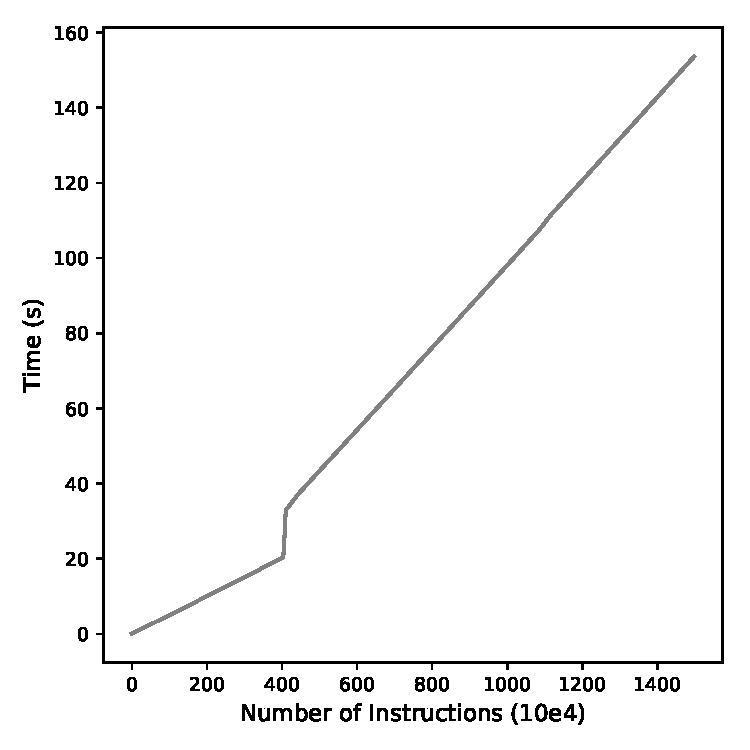
\includegraphics[width=.8\columnwidth]{./figures/result/running_time.pdf}
%    \caption{With the optimization introduced, \tool{} can be scalable to RSA}
%\end{figure}

%\subsubsection{Comparison with the Existing Tools}
\tool{} is designed to quantify side-channel leakages. But it can detect
side-channels leakages as well. In this section, we compare \tool{} with the
existing trace-based side-channel identification tools.

As shown in Table~\ref{eval:cacheD},
\tool{} can not only identify all the leakage sites reported by CacheD~\cite{203878}, but also
many new ones. CacheD fails to detect many other vulnerabilities for two
reasons. First, CacheD can only detect secret-dependent memory access
vulnerabilities. But \tool{} can detect secret-dependent control-flows as well.
Second, CacheD suffers from some performance issues and uses some domain
knowledge to simplify symbolic execution and has to trim the traces before
processing. The design does not introduce false positives, but can neglect some
vulnerabilities. On the contrary, \tool{} does not apply any domain knowledge
and can find more vulnerabilities. The table~\ref{eval:cacheD} shows that
\tool{} is three times faster than CacheD. As the time of symbolic execution
grow quadratically, \tool{} is much faster than CacheD when analyzing the same
number of instructions. For example, when we test~\tool{} on AES from OpenSSL
0.9.7, ~\tool{} is more than 100x faster than CacheD.

Since DATA~\cite{217537} compares several execution traces to identify
side-channel leakages, \tool{} also outperforms DATA in terms of performance.
For example, it takes 234 minutes for DATA to analysis the RSA of implementation
in OpenSSL 1.1.0f. \tool{} only spends 13 minutes according to Table~\ref{table:over_result}.
Also, DATA reports report 278 control-flow and 460 data leaks. Among those leakages,
they found two vulnerabilities. On the contrary, \tool{} can report how many bits is
actually leaked, which eases the pain to discover sensitive leakages.

\begin{table}[]
    \caption{Comparison with CacheD}
    \label{eval:cacheD}
    \resizebox{\columnwidth}{!}{%
        \begin{tabular}{c|c|c|c|ccc}
            \hline
            \multicolumn{1}{l|}{} & \multicolumn{2}{c|}{Number of Instructions} & \multicolumn{2}{c|}{Time (s)} & \multicolumn{2}{c}{Number of Leakages}                                                                                         \\ \cline{2-7}
            \multicolumn{1}{l|}{} & \multicolumn{1}{c|}{CacheD}                 & \multicolumn{1}{c|}{\tool}    & \multicolumn{1}{c|}{CacheD}            & \multicolumn{1}{c|}{\tool}  & \multicolumn{1}{c|}{CacheD} & \multicolumn{1}{c}{\tool} \\ \hline
            AES 0.9.7             & 791                                         & 1,704                         & 43.4                                   & \multicolumn{1}{c|}{0.30}   & \multicolumn{1}{c|}{48}     & 75                        \\
            AES 1.0.2f            & 2,410                                       & 1,350                         & 48.5                                   & \multicolumn{1}{c|}{0.08}   & \multicolumn{1}{c|}{32}     & 88                        \\
            RSA 0.9.7             & 674,797                                     & 16,980,109                    & 199.3                                  & \multicolumn{1}{c|}{1681}   & \multicolumn{1}{c|}{2}      & 105                       \\
            RSA 1.0.2f            & 473,392                                     & 14,468,307                    & 165.6                                  & \multicolumn{1}{c|}{1692}   & \multicolumn{1}{c|}{2}      & 38                        \\ \hline
            Total                 & 1,151,390                                   & 31,451,470                    & 456.8                                  & \multicolumn{1}{c|}{3373.4} & \multicolumn{1}{c|}{84}     & 317                       \\ \hline
            \multicolumn{7}{l}{\# of Instructions per second \qquad  CacheD: 2,519 \qquad \tool: 9,324}                                                                                                                                          \\ \hline
        \end{tabular}
    }
\end{table}

\subsection{Vulnerability Case Study}\label{sec:eval_case}
\subsubsection{AES in mbedTLS}
During our evaluation, we find mbedTLS 2.5 and 2.15.1 have the same
implementation of AES\@. Our tool provides the same leakage report for both
versions. \tool{} identifies that most leakages are in function
\emph{mbedtls\_internal\_aes\_decrypt}. (Other leakage sites are in function
\emph{mbedtls\_aes\_setkey\_enc}.) All leakages are caused by secret-dependent
memory accesses. Shown in Figure~\ref{mbedtls_aes}, there are seven leakage
sites in total. Leakage 1, 2, 3 are the same and leakage 4, 5, 6, 7 are the
same. They both use a pre-computed lookup table to speed up computation.
However, \tool{} reports leakage 1, 2, 3 typically leak more information
compared to leakage 4, 5, 6, 7. We check the source code and find leakage 1, 2,
3 use secret to access the lookup table \emph{RT0, RT1, RT2, RT3}, which is 8K
each. On the contrary, leakage 4, 5, 6, 7 each accesses a smaller lookup table
(2K). Therefore, leakage 4, 5, 6, 7 leak less information.

\begin{figure}%[h!]
    \centering
    \begin{lstlisting}[xleftmargin=.02\textwidth,xrightmargin=.01\textwidth]
int mbedtls_internal_aes_encrypt( mbedtls_aes_context *ctx,
const unsigned char input[16],
unsigned char output[16] )
{
uint32_t *RK, X0, X1, X2, X3, Y0, Y1, Y2, Y3;
...
for( i = ( ctx->nr >> 1 ) - 1; i > 0; i-- )
{
    AES_FROUND( Y0, Y1, Y2, Y3, X0, X1, X2, X3 ); // Leakage 1
    AES_FROUND( X0, X1, X2, X3, Y0, Y1, Y2, Y3 ); // Leakage 2
}
AES_FROUND( Y0, Y1, Y2, Y3, X0, X1, X2, X3 );     // Leakage 3
X0 = *RK++ ^ \                                    // Leakage 4
    ( (uint32_t) FSb[ ( Y0       ) & 0xFF ]       ) ^
    ( (uint32_t) FSb[ ( Y1 >>  8 ) & 0xFF ] <<  8 ) ^
    ( (uint32_t) FSb[ ( Y2 >> 16 ) & 0xFF ] << 16 ) ^
    ( (uint32_t) FSb[ ( Y3 >> 24 ) & 0xFF ] << 24 );
// X1, X2, X3 do the same computation as X0
...                                           // Leakage 5,6,7
PUT_UINT32_LE( X0, output,  0 );
...
return( 0 );
}
\end{lstlisting}
    \vspace*{-6pt}
    \caption{Function \textit{mbedtls\_internal\_aes\_encrypt}}
    \label{mbedtls_aes}
    \vspace*{-9pt}
\end{figure}

\subsubsection{RSA in mbedTLS}
\tool{} identifies several side-channel leakages for the RSA implementation in
MbedTLS. Here we introduce and analyze two cases.
%, as shown in Figure~\ref{fig:mbedtls_rsa_1} and \ref{fig:mbedtls_rsa_2}.

\tool{} reports one bit information is leaked from the branch at line 2 in
Figure~\ref{fig:mbedtls_rsa_1} and it leaks less information than other
leakages. Function \emph{mbedtls\_mpi\_exp\_mod} performs sliding-window
exponentiation for big numbers. The leakage is caused by checking the signed bit
of the big number $N$. Therefore, the leakage can only tell whether $N$ is
greater than zero, which is one bit leak, not severe.

\begin{figure}%[h!]
    \centering
    \begin{lstlisting}[xleftmargin=.02\textwidth,xrightmargin=.01\textwidth]
...
if( mbedtls_mpi_cmp_int( N, 0 ) < 0 || ( N->p[0] & 1 ) == 0 )
    return( MBEDTLS_ERR_MPI_BAD_INPUT_DATA );
...
\end{lstlisting}
    \vspace*{-6pt}
    \caption{Function \textit{mbedtls\_mpi\_exp\_mod}}
    \label{fig:mbedtls_rsa_1}
    \vspace*{-6pt}
\end{figure}

\begin{figure}%[h!]
    \centering
    \begin{lstlisting}[xleftmargin=.02\textwidth,xrightmargin=.01\textwidth]
...
do {
    *d += c; c = ( *d < c ); d++;
}
while( c != 0 );
...
\end{lstlisting}
    \vspace*{-6pt}
    \caption{Function \textit{mpi\_mul\_hlp}}
    \label{fig:mbedtls_rsa_2}
    \vspace*{-6pt}
\end{figure}

Function \emph{mpi\_mul\_hlp}, shown in Figure~\ref{fig:mbedtls_rsa_2},
is notoriously for a series of timing attacks.
Recent patches have fixed many leakages in function \emph{mpi\_mul\_hlp}.
\tool{} reports 8 bits of information is leaked from line 5.
\emph{mpi\_mul\_hlp} is a helper function to perform mbedtls\_mpi
multiplication. As the code will be executed many times, each time it will leak
independent information. The leakage is severe compared to the previous one.

\subsection{Case Study of RSA in OpenSSL} \label{sec::eval_rsa}
For the crypto libraries, it is likely that an updated version has less
vulnerabilities compared to the previous versions because software developers
have patched some of those vulnerabilities.

We test five versions of OpenSSL (0.9.7, 1.0.2f, 1.0.2k, 1.1.0f, 1.1.1). The
result, as shown in Figure~\ref{fig:rsa}, confirms our assumptions. The newer
version of OpenSSL leaked less amount of information compared to the previous
versions. After version 0.9.7g, OpenSSL adopted a fixed-window mod\_exp
implementation for RSA\@. With the new design, the sequence of squares and
multiples and the memory access patterns are independent of the secret key.
\tool{}'s result confirms the new exponentiation implementation has quite
effectively mitigated most of leakages because the other four versions have fewer
leakages than 0.9.7. OpenSSL version 1.0.2f, 1.0.2k and 1.1.0f almost have the
same amount of leakage. We check the changelog and find only one change for
patching vulnerabilities for RSA (CVE-2016-0702). RSA changelog also claims
OpenSSL 1.1.1 adopted ``numerous side-channel attack mitigation.'' The result
confirms our assumptions.

\begin{figure*}
    \centering
    \vspace*{-9pt}
    \hspace*{-8pt}
    \subfloat[RSA OpenSSL 0.9.7]{
        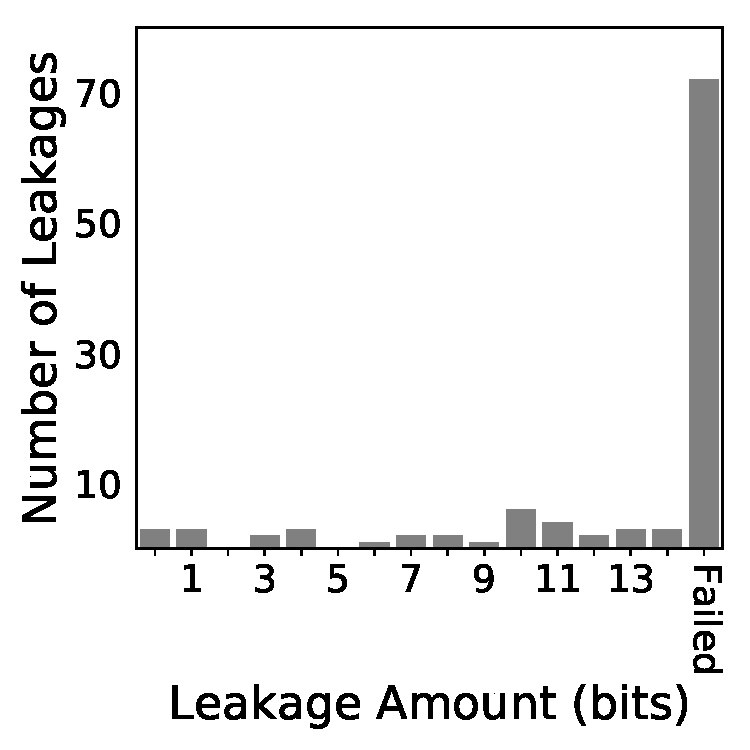
\includegraphics[width=.19\linewidth]{./figures/result/RSA-openssl-0-9-7.pdf}
        \label{fig:rsa-1}
    }
    \subfloat[RSA OpenSSL 1.0.2f]{
        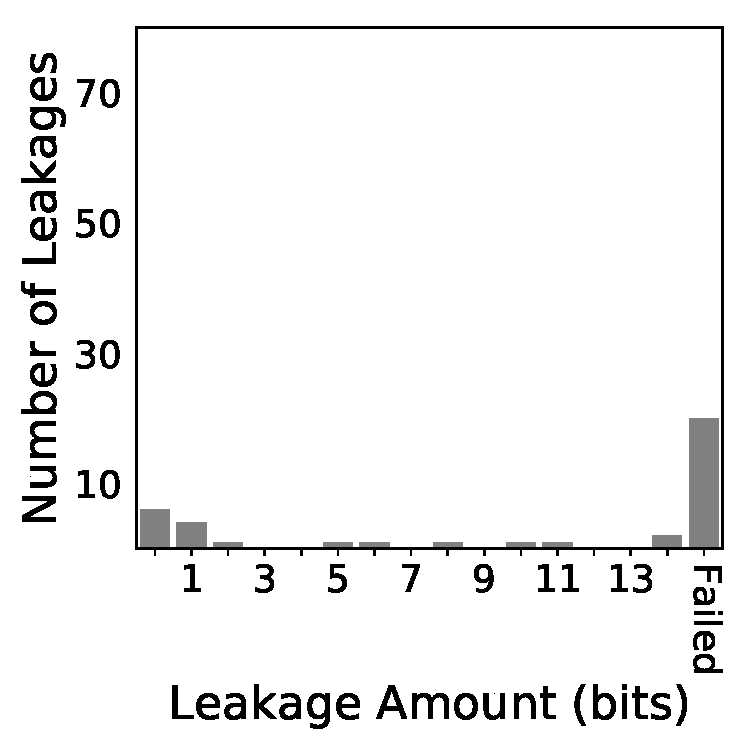
\includegraphics[width=.19\linewidth]{./figures/result/RSA-openssl-1-0-2f.pdf}
        \label{fig:rsa-2}
    }
    \subfloat[RSA OpenSSL 1.0.2k]{
        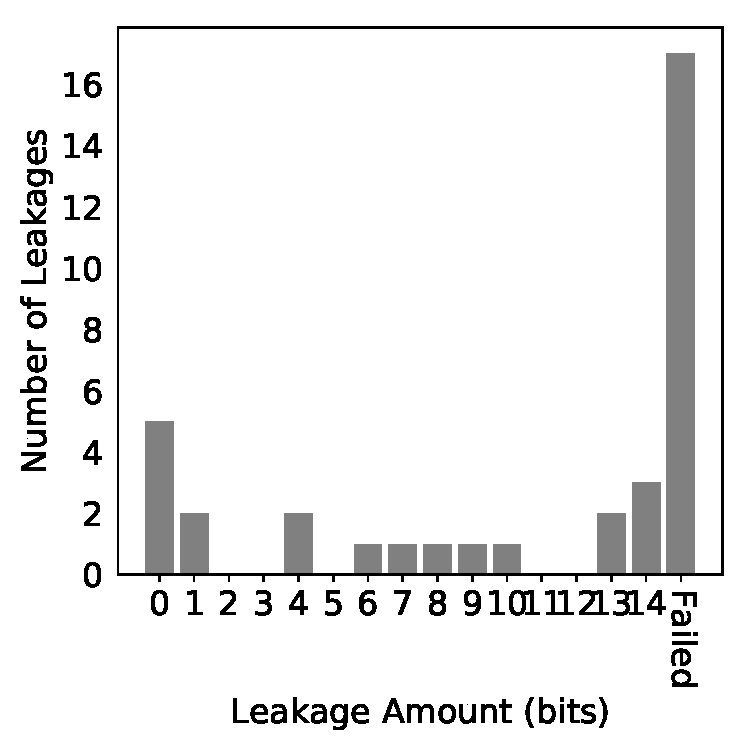
\includegraphics[width=.19\linewidth]{./figures/result/RSA-openssl-1-0-2k.pdf}
        \label{fig:rsa-3}
    }
    \subfloat[RSA OpenSSL 1.1.0f]{
        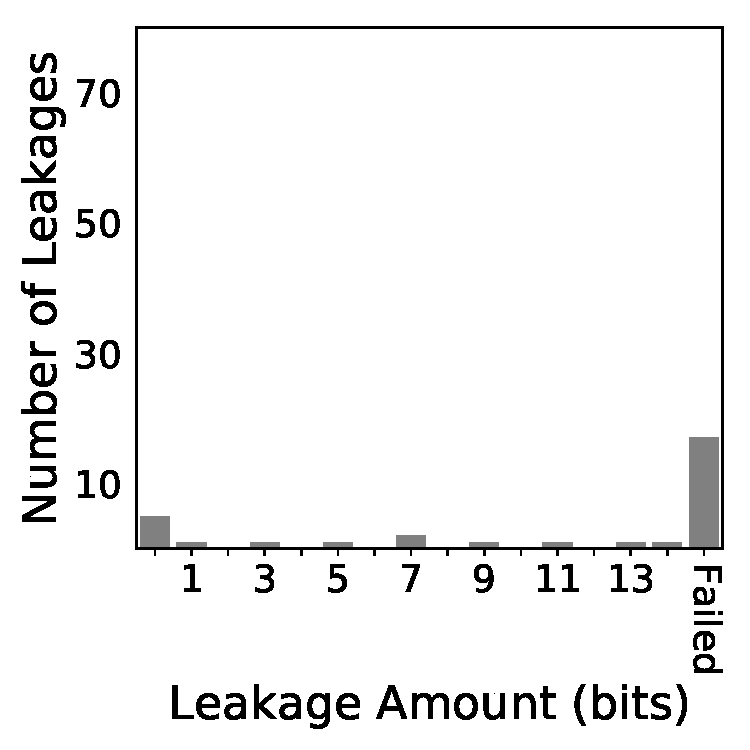
\includegraphics[width=.19\linewidth]{./figures/result/RSA-openssl-1-1-0f.pdf}
        \label{fig:rsa-4}
    }
    \subfloat[RSA OpenSSL 1.1.1]{
        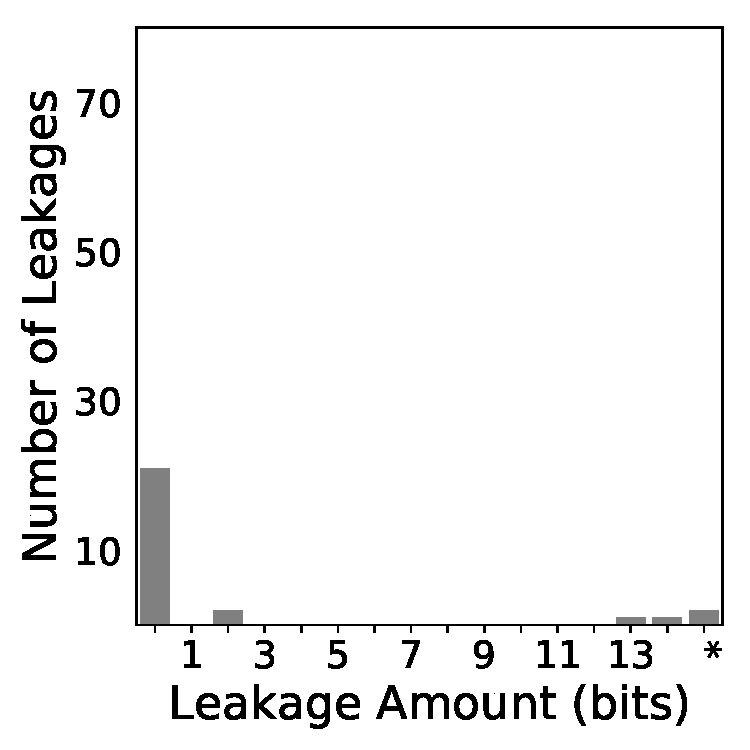
\includegraphics[width=.19\linewidth]{./figures/result/RSA-openssl-1-1-1.pdf}
        \label{fig:rsa-5}
    }
    \caption{RSA implementations in different versions of OpenSSL\@. The mark $*$ means timeout,
        which indicates more severe leakages (see \S\ref{loc:timeout}).}
    \label{fig:rsa}
    \vspace*{-12pt}
\end{figure*}

\subsection{Analysis of Software Countermeasures}\label{sec:eval_countermeasures}
\subsubsection{Bit-slicing}

Bit-slicing is an efficient method to construct constant-time implementation for
side channel to mitigation. The basic concept is to
implement a function in terms of single-bit logical gate operations, such as AND, XOR, OR,
and NOT\@.
% Eli Biham et al.~\cite{Biham:1997:FND:647932.757246} first use gate
% circuits to implement the SBOX of DES\@. Based on his work Matthew
% Kwan~\cite{Kwan2000ReducingTG} present a better implementation of DES with fewer
% gates and first used the term Bit-slicing. 
% This approach can immune cryptographic algorithms to cache and timing-related
% side-channel attacks. 
%Figure~\ref{fig:SBOX_bitslicing} describe a Bit-slicing implement of
%secret-depend Substitution-box (SBOX) shown in Figure~\ref{fig:SBOX_da}.
Since the table lookups and conditional jumps are replaced with single-bit
logical gates, with no secret-dependent memory addresses or control flow, both
the data access and control flow types of side-channel leakages are mitigated.

We would like to test \tool\ on bit-slicing. We adopted the SBOX
implementations, commonly used in block ciphers such as DES and AES, with and
without bit-slicing, and apply \tool\ to confirm the mitigation. The SBOX
implementation with and without bit-slicing are shown in
Figure~\ref{fig:SBOX_bitslicing} and Figure~\ref{fig:SBOX_da}, respectively, in
Appendix~\ref{appendix:SBOX}. Consider an SBOX take some bits derived from a
password as input and output 2-bit transform result. The plain implementation
has a range check on the password input and a secret-dependent table lookup
while bit-slicing does not.
%% The plain implementation will first ensure the input does not overflow
%% and then directly access the table for the substitution result, as described in
%% Figure~\ref{fig:SBOX_da}. While we apply the Bit-sliding to this SBOX, the check
%% and access process will transfer to a series of logical operations described in
%% Figure~\ref{fig:SBOX_bitslicing}.
\tool\ reports that there are both control-flow and data access types of leakage
in the non-bit-slicing implementation
%% We apply \tool to both implementations.
%% According to the result, there exist two leakage sites in non-bit-slicing
%% implementation: one control-flow type leakage from check operation and one data
%% access type leakage from the table lookup operation of directly access method
(line 6 and line 7 in Figure~\ref{fig:SBOX_da}). The number of leaked bits is
5.0 and 4.4, respectively. At line 6, according to Definition~\ref{def}, the
input set $K$ is $[0,2^8-1]$, the observed input set $K^o$ is $[0,2^3-1]$. Thus,
the leakage $L_{\beta(k)\rightarrow o}$ based on the observation ($o$) is
$L_{\beta(k)\rightarrow o} = \log_2{|K|} - \log_2{|K^o|} = 8-3 = 5$ bit, which
confirms the result from \tool. Similarly, we can verify the result of the other
leakage site. \tool{} reports no leakage on the bit-slicing implementation.
% The basic concept is to express a function
% in terms of single-bit logical operations (AND, XOR, OR, NOT, etc.). These
% operations are then carried out for multiple instances of the function in
% parallel, using bitwise operations on a CPU. The original intention of
% Bit-slicing Implementation is to accelerate the crypto algorithms. However,
% thanks to the features of gate operations, the implementations gain additional
% security properties. Since the table lookup operation and conditional jump
% operation will be replaced with single-bit logical gates, without directly
% non-input data access or control flow change, thus both the data access type and
% control flow type of side-channel leakage will be avoided.

% \subsubsection{Scatter and Gather}
% The scatter-gather technology is also a common defence method to cache-based timing attacks.
% \begin{figure}[h!]
%     \centering
%     \begin{lstlisting}[xleftmargin=.02\textwidth,xrightmargin=.01\textwidth]
% ...
% align ( buf ):
%     return buf - ( buf & ( block size - 1 ) ) + block size

% scatter ( buf, p, k ):
%     for i := 0 to N - 1 do
%         buf [k + i * spacing] := p [k][i]

% gather ( r, buf, k ):
%     for i := 0 to N - 1 do
%         r [i] := buf [k + i * spacing]
% ...
% \end{lstlisting}
%     \caption{Scatter\_and\_Gather}
%     \label{Scatter_and_Gather}
% \end{figure}

% \begin{figure}[h!]
%     \centering
%     \begin{lstlisting}[xleftmargin=.02\textwidth,xrightmargin=.01\textwidth]
% ...
% uint8_t SBOX[] = {1, 0, 3, 1, 2, 2, 3, 0};
% align(buf);
% scatter(buf, SBOX, k);
% ...
% \end{lstlisting}
%     \caption{Sbox\_with\_Scatter\_and\_Gather}
%     \label{SBOX_sg}
% \end{figure}

\subsubsection{Smaller Lookup Tables}
Considering the cache-collision timing attack 
\cite{Bonneau11894063_16}, the probability of leakage 
decreases when the lookup table entry or element size is smaller.
So in theory, a lookup table with one-byte size elements
(see Figure~\ref{fig:one_byte_table}) will leak less
information than a table with 4-byte element size
(see Figure~\ref{fig:four_byte_table}).
\tool{} reports one leakage site for each lookup table,
with 12.0 bits for the table with smaller entries and
24.2 bits for the table with bigger entries, confirming the theory.

\section{Discussions and Limitations}
In the section, we discuss \tool's limitations, usages, and some future works.

\tool{} works on the native x86 execution traces. The design, which is very
precise in terms of true leakages compared to other static source code
method~\cite{197207,BacelarAlmeida:2013:FVS:2483313.2483334}, also suffers from
limitations of dynamic approaches as well. \tool{} is not sound and has coverage
problem. Each time we only get one single execution trace. Therefore, we may
neglect some side-channel vulnerabilities on other traces. However, we argue
that it is not a crucial problems for analyzing crypto libraries. Because crypto
libraries are designed to have the same code coverage for various inputs. Our
evaluation also confirms the above point. For symmetric encryptions during our
evaluation, there is no secret-dependent control-flow transfers. RSA
implementations have several secret-dependent control-flow transfers. But after
we manually check those leakages cites. We find most of them are useful for
bound checking, which do not leak much information and have negligible effects
on the whole code coverage as well.

One of the motivations of \tool{} is that while recent works have reported lots
of tentative side-channel vulnerabilities, most of them are unpatched by
developers. Our evaluation result also confirms it. For RSA, the latest
OpenSSL\@ only has one leakage site that can leak more than 3 bits while there
are 22 leakage sites according to \tool{}. DES implementation of OpenSSL\@ has
several sensitive leakages. But given the end life status of DES, it is still
unpatched for the worth of engineering effort. At the early stage of the
project, we hope to find some sensitive leakages but are neglected by
communities for years. But somehow every sensitive leakages identified by
\tool{} are known to people before. We think the main reason is that we only
test famous crypto algorithms in well-known crypto libraries. Those code bases
have been studied for years. So it is unlikely to have unknown sensitive
leakages. We leave the task of applying \tool{} on other libraries and
non-crypto libraries in the future.

%\tool{} works on the native x86 instructions, while some existing
%works~\cite{197207,BacelarAlmeida:2013:FVS:2483313.2483334} find side-channels
%vulnerabilities from source code level or intermediate languages (e.g., VEX,
%REIL). Apart from the scalability issues for IR implementations, \tool{} is
%designed to work on the native x86 instructions for the following
%considerations. First, compliers can introduce or mitigate side channels
%vulnerabilities. For example, the GCC compiler may or may not translate the $!$
%operator into conditional branches. If the branch is secret-dependent, the
%attacker could learn some sensitive information. However, source-based methods
%fail to know how those the machine code looks like, which leads to false
%positives or false negatives.  
%Second, we find many crypto libraries have lots of inlined assembly code. In
%general, it is hard to convert assembly code into source code or IR.



\section{Related Work}

There is a vast amount of work on 
side channel 
detection~\cite{182946, 236338, Brotzman19Casym, 203878,217537,Wichelmann:2018:MFF:3274694.3274741,langley2010ctgrind}, 
  %side channel
mitigation~\cite{Page2005PartitionedCA,
Wang:2007:NCD:1250662.1250723,Zhang:2015:HDL:2775054.2694372,Li:2014:SLH:2541940.2541947,
236344,shih2017t,Coppens:2009:PMT:1607723.1608124,
brickell2006software,crane2015thwarting}, 
and information
quantification~\cite{10.1007/978-3-642-31424-7_40,McCamantE2008,5207642,Phan:2012:SQI:2382756.2382791,Chattopadhyay:2017:QIL:3127041.3127044}, 
Here we only present the closely related work to ours.
Due to space limit, we do not include side channel attack work.

\subsection{Detection}

There are a large number of works on side-channel vulnerability detections in
recent years.  CacheAudit~\cite{182946} uses abstract domains to compute the
over approximation of cache-based side-channel information leakage upper bound.
However, due to over approximation they make, CacheAudit can indicate the
program is side-channel free if the program has zero leakage.  However, it is
less useful to judge the sensitive level of the side-channel leakage based on
the leakage provided by CacheAudit. CacheS~\cite{236338} improves the work of
CacheAudit by proposing the novel abstract domains, which only track
secret-related code. Like CacheAudit, CacheS cannot provide the information to
indicate the sensitive level of side-channel vulnerabilities.
CacheSym~\cite{Brotzman19Casym} introduces a static cache-aware symbolic
reasoning technique to cover multiple paths for the target program. Still, their
approaches cannot assess the sensitive level for each side-channel
vulnerability.

The dynamic approach, usually with taint analysis and symbolic execution,
can perform a very precise analysis. CacheD~\cite{203878} takes a concrete
 execution trace and run the symbolic execution on the top of the trace
to get the formula of each memory address. During the symbolic execution, every
value except the sensitive key uses the concrete value. Therefore, CacheD is
quite precise in term of false positives. We adopted a similar idea to model the
secret-dependent memory accesses. DATA~\cite{217537} detects address-based
side-channel vulnerabilities by comparing different execution traces under
various test inputs. MicroWalk~\cite{Wichelmann:2018:MFF:3274694.3274741} uses
mutual information (MI) between sensitive input and execution state to detect
side-channels. They can only detect control-flow channels and MI scores are less
meaningful for dynamic analysis.

\subsection{Mitigation}
Both hardware~\cite{Page2005PartitionedCA,
Wang:2007:NCD:1250662.1250723,Zhang:2015:HDL:2775054.2694372,Li:2014:SLH:2541940.2541947,
236344} and software~\cite{shih2017t,Coppens:2009:PMT:1607723.1608124,
brickell2006software,crane2015thwarting} side-channels mitigation methods have
been proposed recently. Hardware countermeasures, including parting the hardware
computing resource~\cite{Page2005PartitionedCA}, randomizing cache
accesses~\cite{Wang:2007:NCD:1250662.1250723, 236344}, and designing new
architecture~\cite{tiwari2011crafting}, which need to change the hardware and is
usually hard to adopt in reality. On the contrary, software approaches are
usually easy to implement. Coppens et
al.~\cite{Coppens:2009:PMT:1607723.1608124} introduced a compiler-based approach
to eliminate key-dependent control-flow transfers. Crane et
al.~\cite{crane2015thwarting} mitigated side-channels by randomizing software.
As for crypto libraries, the basic idea is to eliminate key-dependent
control-flow transfers and data accesses. Common approaches include
bit-slicing~\cite{konighofer2008fast,rebeiro2006bitslice} and unifying
control-flows~\cite{Coppens:2009:PMT:1607723.1608124}.

\subsection{Quantification}

Quantitative Information Flow (QIF) aims at providing an information leakage
estimation for the sensitive information given the public output. If zero bit
of the information is leaked, the program is called non-interference. McCamant
and Ernst~\cite{McCamantE2008} quantify the information leakage as the network
flow capacity. Backes et al.~\cite{5207642} proposes an automated method for QIF
by computing an equivalence relation on the set of input keys. But the approach
cannot handle real-world programs with bitwise operations. Phan et
al.~\cite{Phan:2012:SQI:2382756.2382791} propose symbolic QIF. The goal of their
work is to ensure the program is non-interference. They adopt an over
approximation way of estimating the total information leakage and their method
does not work for secret-dependent memory access side-channels.
CHALICE~\cite{Chattopadhyay:2017:QIL:3127041.3127044} quantifies the leaked
information for a given cache behavior. CHALICE symbolically reason about cache
behavior and estimate the amount of leaked information based on cache miss/hit.
Their approach can only scale to small programs, which limits its usage in
real-world applications. On the contrary, \tool{} can assess the sensitive level
of side-channels with different granularities. It can also analyze side-channels
in real-world crypto libraries.




\section{Conclusion}
In this paper, we present a novel information leakage definition and method to
quantify memory-based side-channel leakages. We implement the method in
a prototype called \tool{} and show that it is effective in finding
and quantifying the side-channel leakages. With the new definition of
information leakage that imitates real side-channel attackers, the number of
leaked bits is useful in practice to justify and understand the severity level
of side-channel vulnerabilities. The evaluation results confirm our design goal
and show \tool{} is useful in estimating the amount of leaked information in
real-world applications.


\bibliographystyle{IEEEtran}
\bibliography{refs}

\end{document}


